\chapter{Аппаратные средства}

\section{Схема Тестера}
\label{sec:hardware}

Схема на рисунке~\ref{fig:ttester} основана на схеме Markus F., из проекта AVR Transistortester \cite{Frejek}.
Измененные или перемещенные элементы отмечены \textcolor{green}{зеленым цветом}, дополнительные элементы 
отмечены \textcolor{red}{красным цветом}.\\

Небольшие изменения внесены в электронный выключатель питания, который создавал проблемы в некоторых реализациях. 
Резистор R7 уменьшен до  \(3,3~k\Omega\). Конденсатор C2 уменьшен до \(10~nF\). R8 перенесен так, чтобы вывод порта 
PD6 был подключен к конденсатору C2 через него, а не непосредственно.\\

Дополнительные блокировочные конденсаторы должны быть установлены у выводов питания ATmega и у выводов стабилизатора 
напряжения. 
Добавлен один дополнительный подтягивающий резистор на \(27~k\Omega\) к выводу порта PD7 (вывод 13 ATmega). В этой 
модификации программное обеспечение отключает ВСЕ внутренние подтягивающие резисторы ATmega.\\
 
Добавлен дополнительный кварц на \(8~MHz\) с конденсаторами C11, C12 на \(22~pF\). Точность кварца дает возможность 
более точного измерения времени для того, чтобы измерить ёмкость конденсатора.\\

Новая версия программного обеспечения может использовать переключение масштаба напряжения АЦП. Скорость переключения 
зависит от внешнего конденсатора C1 на AREF (вывод 21 ATmega). Чтобы избежать замедления на величину большую, чем 
необходимо, ёмкость этого конденсатора должна быть уменьшена до \(1~nF\). Можно вообще удалить конденсатор C1.\\
Для адаптации программного обеспечения к конкретной схеме необходимо посмотреть опции в \lname{Makefile} в 
разделе конфигурации~\ref{sec:config} на странице~\pageref{sec:config}. \\

Соотношение резисторов R11/R12 определяет величину напряжения для контроля разряда батареи питания. Я приспособил свое 
программное обеспечение к оригиналу от  Markus F. \cite{Frejek} с величинами резисторов \(10~k\Omega\) и \(3,3~k\Omega\).
Сопротивление резисторов в делителе напряжения можно установить в \lname{Makefile}.\\

Дополнительное опорное напряжение \(2,5~V\), поданное на порт PC4 (ADC4), может использоваться, чтобы проверить и 
откалибровать Тестер на имеющееся напряжение VCC (не обязательно). В качестве ИОН можно использовать LM4040-AIZ2.5 
(0,1\%), LT1004CZ 2.5 (0,8\%) или LM336-Z2.5 (0,8\%).\\

Если не установлен ИОН и не предусмотрена защита с использованием реле, Вы должны установить подтягивающий резистор 
R16 к PC4 с высоким номиналом (\(47~k\Omega\)). Это поможет программному обеспечению обнаружить отсутствующий ИОН. 
Дополнительный интерфейс ISP был добавлен для упрощения загрузки новых версий программного обеспечения.
\begin{figure}[H]
\centering

\includegraphics[width=1.0\textwidth]{../FIG/ttester.pdf}
\caption{Новая схема Тестера}
\label{fig:ttester}
\end{figure}

Таблица~\ref{tab:display-con} показывает назначение портов D для различных дисплеев и дополнительных подключений.
Для интерфейса SPI сигнал LCD-CE присутствует на порту ATmega. Вход сигнала CE (Chip Enable) дисплея также 
может быть подключен к GND вместо подключения его к выходу сигнала LCD-CE ATmega.

\begin{table}[H]
  \begin{center}
    \begin{tabular}{| c || c | c | c | c | c | c |}
    \hline
           & Символьный    & ST7565     & ST7920 LCD     & NT7108 LCD  & SSD1306     & Дополнительная \\
     Порт  & LCD           &   LCD      & serial         & serial      & I\textsuperscript{2}C  & функция \\
    \hline
    \hline
    PD0    &  LCD-D4       &  LCD-REST  & LCD-REST       & 595-PCLK        &            & \\
    \hline
    PD1    &  LCD-D5       &  LCD-RS    &                & LCD-CS2     &             & Энкодер 2 \\
    \hline
    PD2    &  LCD-D6       &  LCD-SCLK  & LCD-B0         & 164-595-CLK &  LCD-SDA    & \\
    \hline
    PD3    &  LCD-D7       &  LCD-SI    &                & LCD-CS1     &             & Энкодер 1 \\
    \hline
    PD4    &  LCD-RS       &            &                & LCD-RS      &             & Внешняя частота \\
           &               &            &                & 164-595-SER &             &                \\
    \hline
    PD5    &  LCD-E        &  (LCD-CE)  & LCD-EN         & LCD-EN      &   LCD--SCL  & \\
    \hline
    PD7    &  кнопка       & кнопка     & кнопка         & кнопка      & кнопка      & \\
    \hline
    \end{tabular}
  \end{center}
  \caption{Назначение контактов порта D для подключения различных дисплеев}
  \label{tab:display-con}
\end{table}

Программное обеспечение может изменять назначение выводов порта D для удобства разводки LCD-дисплея. 
В таблице~\ref{tab:grid-change} показаны варианты подключения для версии Strip Grid и подключения графического 
индикатора к микроконтроллеру ATmega328.
Также указано использование входов портов для дополнительных функций.
При подсоединении графического адаптера к плате версии Strip Grid (опция STRIP\_GRID\_BOARD=1)
функция измерения частоты не может быть использована, потому что порт PD4 (T0) используется.
Но это соединение используется в китайской версии с графическим дисплеем.
В большинстве случаев дополнительные функции, такие как использование энкодера или частотомера проще 
реализовать в версии тестера с символьным дисплеем, потому что все сигналы данных присутствуют в разъеме
подключения дисплея.


\begin{table}[H]
  \begin{center}
    \begin{tabular}{| c || c | c | c | c | c | c |}
    \hline
           & Симв. LCD    & ST7565 LCD & ST7565 LCD    & Допополнительная \\
      Порт &   =1         &   =1       & STRIP\_GRID   & функция \\
    \hline
    \hline
    PD0    &  кнопка      &              &             & \\
    \hline
    PD1    &  LCD-D7      &  LCD-SI      & LCD-A0 (RS) & Энкодер 2  \\
    \hline
    PD2    &  LCD-D6      &  LCD-SCLK    & LCD-REST    & \\
    \hline
    PD3    &  LCD-D5      &  LCD-A0 (RS) & LCD-SCLK    & Энкодер 1 \\
    \hline
    PD4    &  LCD-D4      &  LCD-REST    & LCD-SI      & Внешняя частота \\
    \hline
    PD5    &  LCD-E       &  (LCD-CE)    &             & \\
    \hline
    PD7    &  LCD-RS      &  кнопка      & кнопка      & \\
    \hline
    \end{tabular}
  \end{center}
  \caption{Назначения портов с опцией STRIP\_GRID\_BOARD}
  \label{tab:grid-change}
\end{table}

\section{Улучшения и расширения к прибору}

\subsection{Защита портов ATmega}

Для защиты ATmega вводится один из двух вариантов схемы защиты из представленных на рисунке~\ref{fig:relay_addon}.
В первом варианте контакты обесточенного реле защищают ATmega при отсутствии напряжения питания. Контакты будут разомкнуты программно, 
как только начнется измерение.\\

Во втором варианте защита при помощи диодов уменьшает вероятность повреждения портов ATmega при подключении 
конденсатора с остаточным напряжением.\\

Следует заметить, что ни одна схема не дает полной гарантии защиты ATmega от остаточного заряда конденсатора.
Поэтому, перед тестированием, конденсатор обязательно разрядить!

\begin{figure}[H]
 \begin{subfigure}[b]{.5\textwidth}
  \centering
  \begin{overpic}[width=.78\textwidth]{../FIG/relay_addon.pdf}
  \color{black}
  \put(78,36){\makebox(0,0)[lb]{\footnotesize VCC or Ubat}}  
  \put(78,32){\makebox(0,0)[lb]{\footnotesize depends on  U{\scriptsize реле}}}  
  \end{overpic}
  \caption{с использованием реле}
 \end{subfigure}
  ~
 \begin{subfigure}[b]{.5\textwidth}
  \centering
  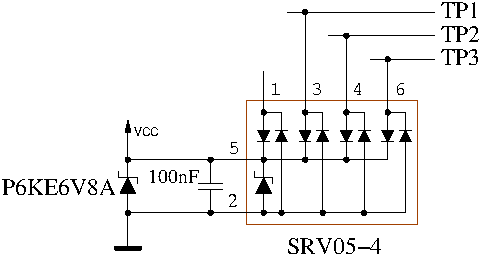
\includegraphics[width=.78\textwidth]{../FIG/diode_addon.pdf}
  \caption{с использованием диодов}
 \end{subfigure}
 \caption{Защита входов ATmega}
 \label{fig:relay_addon}
\end{figure}

Вы можете улучшить защиту, установив реле с тремя группами контактов, как показано на рисунке~\ref{fig:relay_um_addon}.
Разрядный ток ограничен резисторами, входы ATmega отключены в защищенном  режиме. 
Следует помнить, что тестер не защищён в режиме последовательных (циклических) измерений.

\begin{figure}[H]
\centering
 \begin{overpic}[width=.58\textwidth]{../FIG/relay_um_addon.pdf}
  \color{black}
  \put(78,42){\makebox(0,0)[lb]{\footnotesize VCC or Ubat}}  
  \put(78,32){\makebox(0,0)[lb]{\footnotesize depends on  U{\scriptsize реле}}}  
 \end{overpic}
\caption{Улучшенная защита с реле}
\label{fig:relay_um_addon}
\end{figure}

\subsection{Измерение стабилитронов с напряжением более 4 V}

Если UART не требуется, порт PC3 может использоваться в качестве аналогового входа для измерения внешнего напряжения. 
Напряжение может составить до \(50~V\) с дополнительным резистивным делителем 10:1. На рисунке ~\ref{fig:zener} 
представлена схема для измерения напряжение пробоя стабилитрона при низком уровне на порте PD7 ATmega. 
Тестер показывает внешнее напряжение, пока Вы держите кнопку \textbf{ TEST} нажатой. Ток, потребляемый от батареи питания, 
при этом возрастает, примерно, на \(40~mA\).

\begin{figure}[H]
\centering
  \begin{overpic}[width=.90\textwidth]{../FIG/zener_exp.pdf}
  \color{black}
  \put(5,20){\makebox(0,0)[rb]{\textcolor{red}{external}}}  
  \put(5,17){\makebox(0,0)[rb]{\textcolor{red}{Voltage}}}  
  \put(33,24){\makebox(0,0)[rb]{Can be placed on Tester board!}}
  \put(42,2){\makebox(0,0)[lb]{Should be placed separate!}}
 \end{overpic}
\caption{Схема для измерения параметров стабилитронов}
\label{fig:zener}
\end{figure}

Резистивный делитель 10:1 может быть использован для измерения внешних напряжений при выборе из
меню дополнительных функций в ATmega328. Присутствие DC-DC преобразователя для измерения стабилитронов
не мешает, так как кнопка не удерживается в нажатом состоянии и, соответственно, DC-DC преобразователь
обесточен. Таким образом, можно измерять напряжение постоянного тока до \(50~V\) только положительной 
полярности, обязательно соблюдая полярность.\\

\subsection{Генератор частоты}

Из меню дополнительных функций, при использовании ATmega, можно выбрать генератор частоты.
В настоящее время поддерживается выбор частот в диапазоне от \(1~Hz\) до \(2~MHz\). 
Выходной сигнал \(5~V\) через резистор \(680~\Omega\) выводится на тестовый контакт TP2.
В качестве сигнала GND, при этом, можно использовать GND DC-DC преобразователя или тестовый 
контакт TP1. Тестовый контакт TP3 подсоединен к GND через резистор \(680~\Omega\).
Конечно, Вы также можете использовать порт PB2 для подключения отдельной схемы усилителя-формирователя.
Но вход этой схемы не должен создавать большую нагрузку для порта ATmega.\\

\subsection{Измерение частоты}
\label{sec:frequency_counter}

Для использования дополнительной функции измерения частоты, потребуется незначительная 
доработка Тестера. Для измерения частоты используется порт PD4 (T0/PCINT20) ATmega. 
Этот же порт используется для подключения LCD-дисплея. В стандартном варианте к порту PD4 подключен 
сигнал LCD-RS, в варианте strip grid - сигнал LCD-D4. Для обоих сигналов порт PD4 может быть переключен 
на ввод, если в данный момент не требуется выводить информацию на LCD-дисплей.\\
 
Однако, лучше использовать дополнительную схему подключения, изображенную на рисунке~\ref{fig:FreqMes}.
Напряжение на выводе порта PD4 (LCD-RS или LCD-D4) должно быть установлено около \(2,4~V\) при отключенной 
ATmega или подстроено во время измерения частоты ATmega, чтобы получить лучшую чувствительность к входному 
сигналу. Во время регулировки LCD-дисплей должен быть установлен, потому что подтягивающие резисторы 
индикатора могут изменить установленное напряжение.

\begin{figure}[H]
\centering
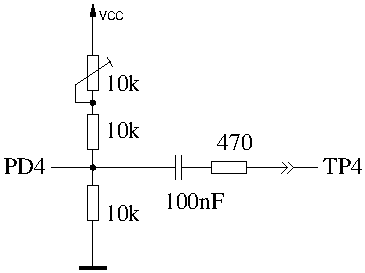
\includegraphics[width=.4\textwidth]{../FIG/Frequency_addon.pdf}
\caption{Дополнительная схема для измерения частоты}
\label{fig:FreqMes}
\end{figure}

\subsection{Использование поворотного энкодера}

Для более удобного доступа к Меню дополнительных функций для ATmega328, Вы можете дополнить схему, установив
инкрементальный энкодер с кнопкой.   
Рисунок~\ref{fig:RotExt} показывает схему подключения к тестеру с символьным LCD.
Все сигналы для подключения поворотного инкрементального энкодера доступны в разъеме 
подключения LCD. По этому, модернизация возможна для большинства существующих тестеров.
Во многих случаях графический LCD собран на переходной плате и подключен к контактам, предназначенным
для подключения символьного LCD. Таким образом, модернизация в этих случаях также возможна.    

\begin{figure}[H]
\centering
 \begin{overpic}[width=.30\textwidth]{../FIG/rotary_extension.pdf}
  \color{black}
%  \put(47,6){\makebox(0,0)[lb]{Taster}}    
 \end{overpic}
\caption{Схема подключения поворотного энкодера}
\label{fig:RotExt}
\end{figure}

На рисунке~\ref{fig:RotEnc} показана особенность работы двух типов поворотных инкрементальных 
энкодеров.
В версии 1 полная последовательность состояния переключателей происходит при повороте на два 
фиксированные положения. Количество полных циклов в два раза меньше чем количество фиксированных
положений за оборот энкодера.
В версии 2 при повороте на одно фиксированное положение генерируется полный цикл состояния контактов. 
В этом случае количество фиксированных положений соответствует количеству циклов за оборот энкодера.  
Иногда, в таких энкодерах, в каждом фиксированном положении состояние переключателей всегда 
одинаково.
\begin{figure}[H]
\centering
 \begin{overpic}[width=.87\textwidth]{../FIG/rotary_encoder.pdf}
  \color{black}
  \put(90,71.5){\makebox(0,0)[lb]{тумблер A}}
  \put(90,62){\makebox(0,0)[lb]{тумблер B}} 
  \put(90,29){\makebox(0,0)[lb]{тумблер A}}
  \put(90,19){\makebox(0,0)[lb]{тумблер B}}
  \put(6,6){\makebox(0,0)[rb]{\footnotesize состояние}}    
  \put(6,48.5){\makebox(0,0)[rb]{\footnotesize состояние}}    
  \multiput(23.5,53)(24.6,0){3}{\footnotesize стопор}
  \multiput(11,10)(12.3,0){6}{\footnotesize стопор}
  \put(52,43){\makebox(0,0)[cb]{{\large версия 2}}}
  \put(52,1){\makebox(0,0)[cb]{{\large версия 1}}}      
 \end{overpic}
 \caption{Особенности двух типов поворотных инкрементальных энкодеров}
 \label{fig:RotEnc}
\end{figure}
Рисунок~\ref{fig:RotBounce} показывает работу энкодера, который имеет не только \inquotes{дребезг} контактов
но и неустойчивое состояние переключателя в точке фиксации. Каждое изменение 
состояния переключателей определяется программой и сохраняется в циклический буфер.
Поэтому, последние три состояния переключателей можно проверить после каждого изменения состояния.
Для каждого цикла переключения состояний, в общей сложности четыре последовательности могут быть 
определены для каждого направления вращения.

Если за одну фиксированную позицию осуществляется один, полный, цикл состояний переключателей, то для правильного
подсчета достаточно контролировать состояние переключателя в одном канале (WITH\_ROTARY\_SWITCH=2 или 3).

Если для генерации полного цикла состояний переключателей требуется поворот на две фиксированные
позиции, как показано на рисунке~\ref{fig:RotBounce}, Вы должны контролировать последовательность
переключения в двух каналах (WITH\_ROTARY\_SWITCH=1).

Для энкодеров без фиксации, Вы можете выбрать любую чувствительность к углу поворота. Значение 
2 и 3 устанавливает низкую чувствительность, 1 среднюю чувствительность и 5 высокую чувствительность.

Подсчет импульсов (количество \inquotes{вверх}, количество \inquotes{вниз}) может быть обеспечен подбором 
определенного алгоритма, но, в то же время, может быть утрачен из-за неустойчивого состояния 
контактов переключателей в точке фиксации.
\begin{figure}[H]
\centering
 \begin{overpic}[width=.87\textwidth]{../FIG/rotary_bouncing.pdf}
  \color{black}
  \put(90,39){\makebox(0,0)[lb]{окошечко A}}
  \put(90,30){\makebox(0,0)[lb]{окошечко B}}
  \multiput(12,23)(28,0){3}{\footnotesize защелка}
  \put(7,20){\makebox(0,0)[rb]{состояние}}
  \put(5,12){\makebox(0,0)[lb]{Возможные состояния слева направо:}}      
 \end{overpic}
	\caption{Энкодер с \inquotes{дребезгом} контактов переключателей}
 \label{fig:RotBounce}
\end{figure}	
Если энкодер не доступен или не целесообразен из-за конструктивных соображений, вместо двух контактов энкодера, 
Вы можете подсоединить две независимые кнопки для перемещения \inquotes{Вверх} и \inquotes{Вниз}.
В этом случае значение опции WITH\_ROTARY\_SWITCH, для корректной работы программы, должно быть установлено 4.

\subsection{Подключение графического дисплея}

Большое спасибо Wolfgang Sch. за выполненную работу по поддержке прибором китайской версии дисплея с контроллером ST7565.
В настоящее время вы также можете подключить графический LCD (128x64 пикселей) с контроллером ST7565. 
Поскольку контроллер ST7565 подключается по последовательному интерфейсу, то только четыре сигнальных
линии используется. Два вывода порта D ATmega могут быть использованы для других задач.
ATmega процессор должен иметь, по крайней мере, \(32~kB\) флеш-памяти для поддержки графического дисплея.
ST7565 контроллер использует рабочее напряжение \(3,3~V\).
Поэтому требуется дополнительный стабилизатор \(3,3~V\).
Документация к контроллеру ST7565 не допускает прямого подключения логических 
сигналов уровня \(5~V\). Для согласования логических уровней сигналов \(5~V\) и \(3,3~V\) можно использовать
схему, приведенную на рисунке~\ref{fig:ST7565lcd} с использованием 
микросхемы преобразователя уровней 74HC4050.
Вы можете попробовать применить вместо четырех элементов 74HC4050 четыре резистора, примерно \(2,7~k\Omega\).
Падение напряжения на резисторах предотвратит увеличение напряжения на входах графического контроллера больше чем
напряжение питания \(3,3~V\), а дополнительные диоды на входах графического контроллера не допустят попадания 
выходного сигнала \(5~V\) от ATmega.
Вы должны убедиться, что форма сигналов с резисторов могут быть правильно восприняты входами контроллера ST7565.
 
В любом случае, при применении элементов микросхемы 74HC4050 форма сигнала на входе графического контроллера 
точнее соответствует форме выходного сигнала с ATmega. 

\begin{figure}[H]
\centering
 \begin{overpic}[width=.814\textwidth]{../FIG/ST7565lcd.pdf}
  \color{black}
  \put(88,10){\makebox(0,0)[lb]{Background}}
  \put(88,7){\makebox(0,0)[lb]{LED}}
 \end{overpic}
\caption{Подключение графического дисплея с контроллером ST7565}
\label{fig:ST7565lcd}
\end{figure}

В таблице~\ref{tab:spi-processor} показаны другие альтернативы подключения ATmega328 
или других микроконтроллеров по интерфейсу SPI (LCD\_INTERFACE\_MODE=4) или для трехпроводного
соединения (LCD\_INTERFACE\_MODE=3).
Различные типы подсоединений для одного типа процессора могут быть выбраны с помощью опции
в \lname{Makefile} STRIP\_GRID\_BOARD.
Назначение контактов разъема определено в файле \lname{config.h}.
Если Вам нужно иное подключение, Вы должны назначить новый номер кода для 
опции STRIP\_GRID\_BOARD и задать настройку подключения в файле \lname{config.h}.

\begin{table}[H]
  \begin{center}
    \begin{tabular}{| c || c | c | c | c | c | c | c |}
    \hline
 Контроллер  & m644  & m1280 & m1280  & m328 & m328 & m328 & m328 \\
STRIP\_GRID\_BOARD &       &   -   &   1    &  -   &  1   &  2   &  5   \\
Сигнал:     &       &       &        &      &      &      &     \\
    \hline
    \hline
  RES       &  PB4  & PA0   &  PA4   & PD0  & PD4  & PD0  & PD2 \\
    \hline
  EN, CLK   &  PB6  & PA2   &  PA2   & PD2  & PD2  & PD2  & PD3 \\
    \hline
  RS, D/C   &  PB5  & PA1   &  PA3   & PD1  & PD3  & PD3  & PD1 \\
    \hline
  B0, MOSI  &  PB7  & PA3   &  PA1   & PD3  & PD1  & PD1  & PD4 \\
    \hline
  CE, CS    &  PB3  & PA4   &  PA5   & PD5  & PD5  & PD5  & PD5 \\
    \hline
    \end{tabular}
  \end{center}
  \caption{Подключение по SPI для различных контроллеров}
  \label{tab:spi-processor}
\end{table}

Обычно ST7565 или SSD1306 контроллер подключается по 4-проводному SPI интерфейсу.
Но с контроллером SSD1306 Вы также можете подключить индикатор по интерфейсу I\textsuperscript{2}C использовав PD2 
как SDA и PD5 как SCL сигнал.
Сигналы SDA и SCL должны быть подтянуты резисторами около \(4,7~k\Omega\) к напряжению \(3,3~V\).
Пример подключения OLED дисплея показан на рисунке~\ref{fig:ssd1306i2c}.
Сигналы шины I\textsuperscript{2}C реализованы только путем переключения портов ATmega к \(0~V\).
Перед подключением подтягивающих резисторов к напряжению \(5~V\), Вы должны убедиться, что Ваш контроллер
допускает уровень сигнала \(5~V\). Обычно входы контроллера дисплея защищены диодами, которые понижают уровень 
сигнала до \(3,3~V\). 
Вы должны убедиться, что в ATmega записана программа с поддержкой интерфейса I\textsuperscript{2}C до того,
как дисплей будет подсоединен. Если Вы записали в контроллер микропрограмму с поддержкой другого интерфейса,
то на выводах ATmega могут присутствовать сигналы с уровнем \(5~V\).

Так, как я обнаружил влияние на результаты теста модуля OLED через шину \(VCC\), рекомендую
установить дополнительную развязку из последовательного резистора \(68~\Omega\) и разделительного конденсатора \(10~\mu F\). 
Вместо \(68~\Omega\) резистора можно также использовать индуктивность \(1~mH\).
Без дополнительного фильтра мой тестер с дисплеем OLED определял остаточные токи в коллекторах биполярных транзисторов.

Также нужно проверить расположение выводов Вашего OLED дисплея. Некоторые модули имеют отличие в расположении \(GND\) и \(VCC\).   
 
\begin{figure}[H]
\centering
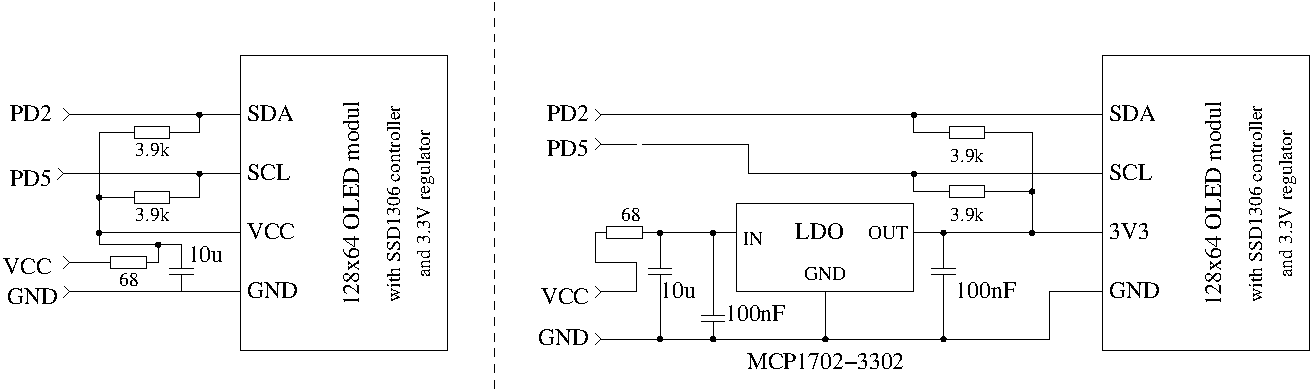
\includegraphics[width=.814\textwidth]{../FIG/SSD1306_I2C.pdf}
\caption{Подключение графического OLED дисплея с I\textsuperscript{2}C интерфейсом}
\label{fig:ssd1306i2c}
\end{figure}

Для подключения к контроллерам серии ATmega644 вместо портов PB3 (SCL) и PB4 (SDA) используются порты PD5 и PD2.
Для микроконтроллеров серии ATmega1280 используются контакты PA5 (SCL) и PA4 (SDA).
Для замены символьного дисплея на графический можно использовать переходную печатную плату-адаптер с разъемом
аналогичным символьному LCD, так как все сигналы и питание на нем доступны.

Намного проще подключить дисплей с контроллером ST7920, потому что контроллер поддерживает напряжение питания \(5~V\).
Дисплей должен поддерживать режим 128x64 точек.
Модуль дисплея с контроллером ST7920 может быть подключен по 4-bit параллельному интерфейсу или по специальному,
последовательному интерфейсу, согласно рисунка~\ref{fig:ST7920lcd}.

\begin{figure}[H]
\centering
 \begin{overpic}[width=.698\textwidth]{../FIG/ST7920interface.pdf}
  \color{black}
  \put(20,1){\makebox(0,0)[cb]{serial mode}}  
  \put(80,1){\makebox(0,0)[cb]{4-bit parallel mode}}   
 \end{overpic}
\caption{Подключение индикатора с контроллером ST7920}
\label{fig:ST7920lcd}
\end{figure}

Для двух типов подключения индикатора с контроллером ST7920 в \lname{Makefile} должна быть установлена опция 
\inquotes{WITH\_LCD\_ST7565 = 7920}. Кроме того, при подключении по последовательному интерфейсу, 
надо установить и опцию \inquotes{CFLAGS += -DLCD\_INTERFACE\_MODE=5}.

В таблице~\ref{tab:ser-processor} показано подключение различных микроконтроллеров по
последовательному интерфейсу с опциями INTERFACE\_MODE 5 (ST7920) и 7 (SSD1803).

\begin{table}[H]
  \begin{center}
    \begin{tabular}{| c || c | c | c | c |}
    \hline
 Контроллер  & m644  & m644 & m1280  & m328 \\
STRIP\_GRID\_BOARD &   -   &   1   &        &     \\
Сигнал:     &       &       &        &         \\
    \hline
    \hline
  EN        &  PB3  & PB6   &  PA5   & PD5     \\
    \hline
  B0, R/W   &  PB4  & PB7   &  PA4   & PD2      \\
    \hline
  RESET     &  PB2  & PB4   &  PA0   & PD0      \\
    \hline
    \end{tabular}
  \end{center}
  \caption{Порты для последовательного подключения различных контроллеров}
  \label{tab:ser-processor}
\end{table}

Так же как и в случае применения других графических индикаторов, для дисплея с контроллером ST7920,
опциями LCD\_ST7565\_H\_FLIP и LCD\_ST7565\_V\_FLIP можно изменить ориентацию выводимого изображения.

Особым случаем является подключение дисплеев с контроллером NT7108 (KS0108, S6B0108). Поскольку эти дисплеи 
используют только параллельный 8-битный интерфейс, необходимо применение последовательно - параллельного 
преобразователя интерфейсов. Простейший способ -- использование микросхемы 74HCT164 или 74HCT595.
Вариант такого подключения показан на рисунке~\ref{fig:NT7108lcd}.

\begin{figure}[H]
  \begin{subfigure}[b]{.5\textwidth}
    \centering
    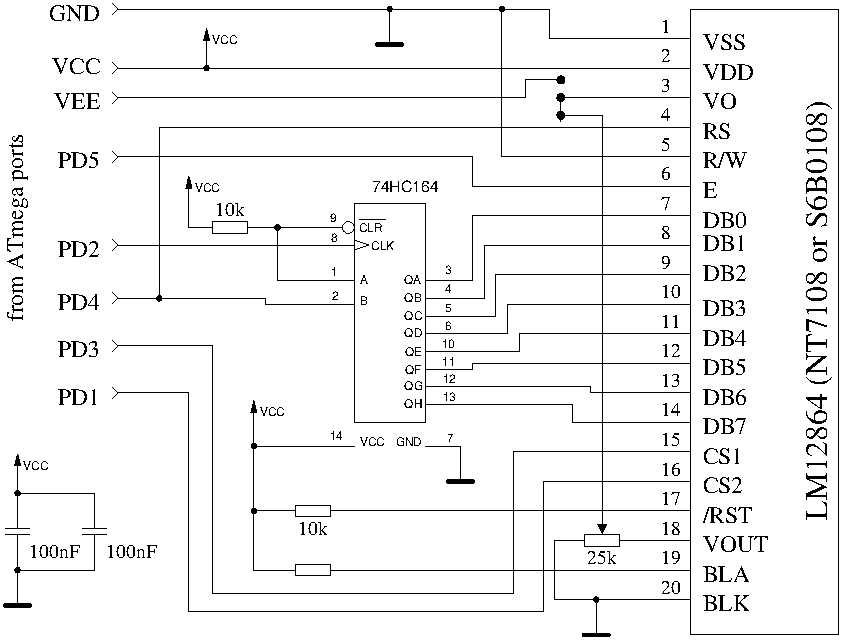
\includegraphics[width=.9\textwidth]{../FIG/ST7108serial164.pdf}
    \caption{с использованием 74HCT164}
  \end{subfigure}
  ~
  \begin{subfigure}[b]{.5\textwidth}
    \centering
    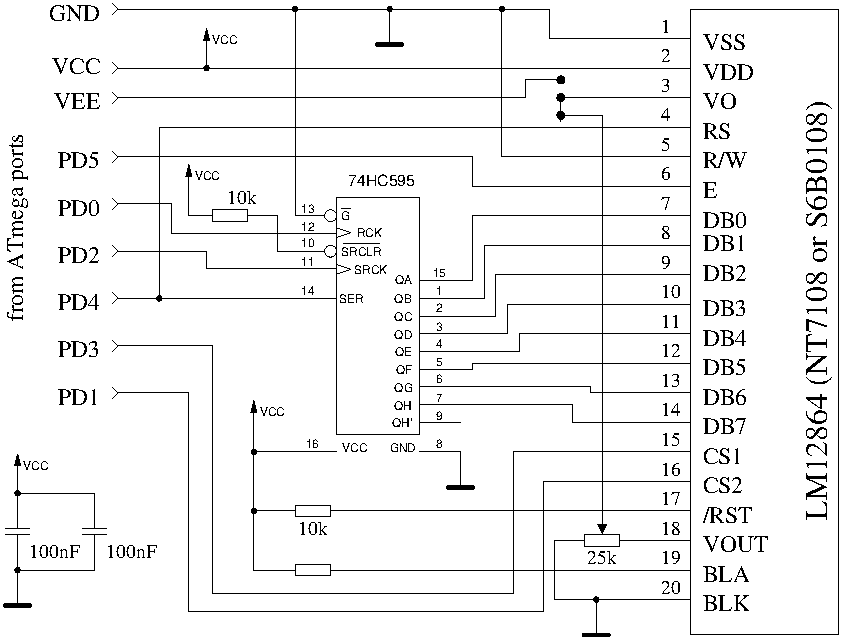
\includegraphics[width=.9\textwidth]{../FIG/ST7108serial595.pdf}
    \caption{с использованием 74HCT595}
  \end{subfigure}
  \caption{Подключение графического дисплея с NT7108 контроллером}
  \label{fig:NT7108lcd}
\end{figure}

Так как некоторые модули LCD различаются по расположению выводов, перед подключением Вы должны проверить цоколёвку 
Вашего дисплея. 
Некоторые различия в расположении выводов для серии LCD ABG128064 приведены в таблице~\ref{tab:NT7108types}.

\begin{table}[H]
  \begin{center}
    \begin{tabular}{| c || c | c | c | c |}
    \hline
           & 128064H  &  128064G  & 128064C  & 128064B \\
    Сигнал &         &          &         &         \\
    \hline
    \hline
  VDD (5V) &   1     &  2       &   4     & 2       \\
    \hline
  VSS (GND) &   2     &  1       &   3     & 1       \\
    \hline
 VO (Drive) &   3     &  3       &  (5)    & 3       \\
    \hline
  DB0-DB3   &   4-7   &  7-10    &   9-12  & 7-10    \\
    \hline
  DB4-DB7   &   8-11  &  11-14   &   13-16 & 11-14   \\
    \hline
  CS1       &   12    &  15      &   1     & 15      \\
  CS2       &   13    &  16      &   2     & 16      \\
    \hline
  Reset     &   14    &  17      &   -     & 17      \\
    \hline
  R/W       &   15    &  5       &   7     & 5       \\
    \hline
  RS        &   16    &  4       &   6     & 4       \\
    \hline
  E         &   17    &  6       &   8     & 6       \\
    \hline
  VEE       &   18    &  18      &   -     & 18      \\
    \hline
  LEDA      &   19    &  19      &   17    & (19)      \\
  LEDK      &   20    &  20      &   18    & -      \\
    \hline
    \end{tabular}
  \end{center}
  \caption{Различие в цоколёвке NT7108 модулей}
  \label{tab:NT7108types}
\end{table}

В таблице~\ref{tab:7108-processor} показано подключение по последовательному интерфейсу индикаторов 
NT7108 к различным микроконтроллерам.
\begin{table}[H]
  \begin{center}
    \begin{tabular}{| c || c | c | c |}
    \hline
Контроллер  & m644  &  m1280  & m328 \\
Сигнал:     &       &        &         \\
    \hline
    \hline
  EN        &  PB3  &  PA5   & PD5     \\
    \hline
  RS        &  PB2  &  PA4   & PD4      \\
  B0        &  PB2  &  PA4   & PD4      \\
    \hline
  CS1       &  PB7  &  PA3   & PD3      \\
    \hline
  CS2       &  PB5  &  PA1   & PD1      \\
    \hline
  CLK       &  PB6  &  PA2   & PD2      \\
    \hline
  PCLK      &  PB4  &  PA0   & PD0      \\
    \hline
    \end{tabular}
  \end{center}
  \caption{Подключение индикаторов с NT7108 по последовательному интерфейсу}
  \label{tab:7108-processor}
\end{table}

Вы также можете использовать дисплей с контроллером PCF8814, который обычно используется, 
например, в Nokia 1100. 
Вы должны проверить, какой интерфейс контроллера используется в Вашем модуле дисплея.
Контроллер PCF8814 может поддерживать SPI-интерфейс 3-х проводной или 4-х проводной, 
I\textsuperscript{2}C-интерфейс и специальный 3-х проводной, который ждёт сигнал 
данные/команда в качестве первого бита в 8 битных данных.
Потому, что дисплей поддерживает только 96х65 пикселей, большие иконки для транзисторов не используются 
с этим контроллером. Вывод результатов похож на вывод для символьных дисплее. 
Как и большинство графических дисплеев, этот контроллер работает с \(3,3~V\). 
Поэтому требуется преобразователь уровней логических сигналов для \(5~V\) выходов ATmega.
Для SPI интерфейса и 3-х проводного интерфейса Вы можете использовать опцию в \lname{Makefile}
LCD\_SPI\_OPEN\_COL (\inquotes{открытый коллектор} портов ATmega).
Вы должны использовать \inquotes{Pull-Up} резисторы или не устанавливать 
опцию PULLUP\_DISABLE в \lname{Makefile}.  
В настоящее время с контроллером PCF8814 протестирован только 3-х проводной интерфейс.

\begin{table}[H]
  \begin{center}
    \begin{tabular}{| c || c | c | c | c |}
    \hline
     Порт  &  PCF8814    & PCF8814        & PCF8814     & Дополнительная \\
           &    SPI      & 3-х проводной  & I\textsuperscript{2}C  & функция \\
    \hline
    \hline
    PD0    &   LCD-RESet  & LCD-RESset       &            & \\
    \hline
    PD1    &   LCD-D/C   & LCD-SCE        &             & Энкодер 2 \\
    \hline
    PD2    &   LCD-SCLK  & LCD-SCLK       &  LCD-SDIN   & \\
    \hline
    PD3    &   LCD-SDIN  & LCD-SDIN       &             & Энкодер 1 \\
    \hline
    PD4    &             &                &             & Внешняя частота \\
    \hline
    PD5    &             & LCD-EN         &   LCD-SCLK  & \\
    \hline
    \end{tabular}
  \end{center}
  \caption{Назначение контактов для различных типов интерфейсов контроллера PCF8814}
  \label{tab:PCF8814-con}
\end{table}

Исходный код для поддержки контроллера PCF8812 с 102x65 пикселей также реализован, 
но, пока, не тестировался.

\subsection{Подключение графического цветного дисплея}

В предложениях китайских продавцов встречаются дешевые модули цветных дисплеев с интерфейсом SPI.
На рисунке~\ref{fig:Color_both} показан вид сзади двух поддерживаемых дисплеев с 128x128 и 
128x160 пикселей.
Размер модулей очень мал, поэтому текст и символы очень мелкие.
Но, в целом, внешний вид четкий и ясный.

\begin{figure}[H]
\centering
\includegraphics[width=.46\textwidth]{../PNG/Color_ILI9163_ST7735.jpg}
\caption{Вид сзади двух цветных LCD}
\label{fig:Color_both}
\end{figure}

Модуль 128x128 пикселей использует контроллер ILI9163.
Модуль 128x160 пикселей использует контроллер очень близкий к ST7735 контроллеру.
Модули тестировались с платой адаптера, которая соединяет сигналы SPI и питание выводов для 
нормального отображения символов. Адаптация выходных уровней \(5~V\) сигналов ATmega к уровню \(3,3~V\) 
сигналов входов контроллера обеспечивается последовательными \(10 k\Omega\) резисторами.
Наличие подсветки (LED) обязательно, т.к. без нее выводимую информацию невозможно прочесть.
Из-за высокого разрешения по вертикали можно отобразить несколько текстовых строк в этих модулях.
Для дисплея 128x128 пикселей можно отобразить 8 строк текста шрифтом 12x8,
для дисплея 128x160 пикселей получим 10 строк текста.
На рисунке~\ref{fig:Color_PNP} Вы можете видеть результат измерения германиевого транзистора
на дисплее 128x128 пикселей.

\begin{figure}[H]
\centering
\includegraphics[width=.46\textwidth]{../PNG/Color_PNP_ILI9163.jpg}
\caption{Измерение биполярного PNP транзистора}
\label{fig:Color_PNP}
\end{figure}

Цветность модулей в настоящее время не используется.
Цвет фона и цвет отображаемых элементов можно изменить в файле lcd\_defines.h или
в \lname{Makefile}.
Контроллер использует программное 16-битное управление цветностью. Цвет отображаемой информации может 
быть изменен параметром LCD\_FG\_COLOR, а цвет подсветки параметром LCD\_BG\_COLOR .



\section{Указания по сборке Тестера }

В Тестере может использоваться LCD-дисплей 2x16, программно совместимый с HD44780 или ST7036. Вы должны учитывать ток, 
необходимый для подсветки, некоторым LCD-дисплеям нужен ток ниже, чем другим. Я пытался применить OLED-дисплей, но он 
стал причиной помех при измерениях для ATmega, и я его \textbf{ не} рекомендую. Также использование OLED-дисплея вызвало 
проблему загрузки специального символа для отображения резистора.\\

Чтобы получить максимальную точность измерения, резисторы R1 - R6 \(680~\Omega\) и
\(470~k\Omega\) должны быть точными (0,1\%). В Тестере могут использоваться ATmega8, ATmega168 и ATmega328. Для 
возможности использовать все функции, рекомендуется установить ATmega328.\\
 
Сначала Вы должны собрать все элементы Тестера на печатной плате без микроконтроллера. В качестве IC2 рекомендуется 
использовать стабилизатор с малым падением напряжения MCP1702-5002, потому что он потребляет всего  \(2~\mu A\) и может 
выдавать \(5~V\) при входном напряжение всего \(5,4~V\). Но он несовместим по выводам с известным 78L05 в корпусе TO92 .\\

После проверки правильности монтажа, необходимо подсоединить батарею или источник питание к плате без LCD-дисплея и 
микроконтроллера. При нажатой кнопке \textbf{ TEST} должно присутствовать напряжение \(5~V\) на выводах питания 
микроконтроллера и LCD дисплея. Если отпустить кнопку \textbf{ TEST}, напряжение должно исчезнуть. Если  напряжения 
в норме, то необходимо отключить питание, \textbf{ правильно} вставить микроконтроллер и подключить LCD-дисплей. 
Перед подключением LCD дисплея необходимо 
внимательно проверить правильность соединения выводов питания LCD дисплея (т.к. на некоторых LCD дисплеях они 
подключены наоборот) с GND и VCC платы Тестера!\\
 
Если Вы уверены, что все в порядке, можно подсоединить питание. Если Вы уже запрограммировали ATmega, то можете 
кратковременно нажать кнопку \textbf{ TEST}. При кратковременном нажатии кнопки \textbf{ TEST} светодиод LED1 и подсветка 
LCD-дисплея должны включиться. 
Если Вы отпускаете кнопку \textbf{ TEST}, светодиод LED1 не должен гаснуть как минимум несколько секунд 
(зависит от установленных параметров при компилляции программного обеспечения). 
Заметьте, что программное обеспечение для микроконтроллера должно быть для используемого типа микроконтроллера. Программа для ATmega8 не работает на ATmega168!


\section{Доработки для версий Тестера Markus F.}
\label{sec:change_markus}
\begin{description}

\item[Контроль напряжения.]
Проблема проявляется следующим образом: Тестер немедленно отключается при каждом включении. Причиной может стать 
установка фьюзов (\lname{Makefile}) контроля за понижением напряжения питания ATmega на \(4,3~V\). Происходит это следующим 
образом: порт PD6 пытается зарядить конденсатор C2 \(100~nF\) до уровня VCC, что вызывает провал напряжения 
VCC (\(5~V\)). Для решения проблемы конденсатор C2 может быть уменьшен до \textless~\(10~nF\). Если возможно, 
то включить последовательно в цепь PD6  резистор сопротивлением более \textgreater~\(220~\Omega\).
\item[Улучшение питания схемы.]
Если Тестер запускается при нажатии на кнопку \textbf{ TEST}, но ключ сразу же отпускается, то часто причина этой проблемы 
в питании. Проблема порождена большим током подсветки LCD-дисплея. Резистор R7 к базе P-N-P-транзистора T3 был 
величиной \(27~k\Omega\), 
чтобы уменьшить потребление энергии. Чтобы улучшить переключение при  более низком напряжении батареи или при низком 
коэффициенте усиления P-N-P транзистора T3, необходимо уменьшить сопротивление до \(3,3~k\Omega\).
\item[Дополнительный подтягивающий резистор порта PD7.]
Отсутствие подтягивающего резистора, после короткого времени, работа заканчивается  выключением Тестера с сообщением 
\inquotes{Timeout}. Программное обеспечение формируется с опцией PULLUP\_DISABLE, т. е. все внутренние подтягивающие резисторы 
отключены. По этой причине напряжение порта PD7 не определено, если уровень не переключен кнопкой \textbf{ TEST} или 
транзистором T2 к GND. Внешний резистор сопротивлением \(27~k\Omega\) к VCC решает эту проблему.
\item[Конденсатор C1 в AREF.]
Многие используют на контакте AREF конденсатор на \(100~nF\) так же, как и Markus F. Пока не было необходимости менять 
опорное напряжение АЦП - это было хорошим решением. Программное обеспечение для ATmega168 и ATmega328 использует 
автоматический выбор внутреннего опорного напряжения АЦП \(1,1~V\), если входное напряжение ниже \(1~V\). Это позволяет 
улучшить разрешение АЦП при небольших входных напряжениях. К сожалению, переключение опорного напряжения от \(5~V\) до 
\(1,1~V\) происходит очень медленно. По этой причине нужно учитывать дополнительное время ожидания \(10~ms\). 
При уменьшении величины конденсатора до \(1~nF\), это время может быть существенно уменьшено. Я не заметил ухудшения 
качества измерения при этом изменении. Даже с удалённым конденсатором нет существенного изменения результатов 
измерения. Если Вы предпочитаете оставить конденсатор на \(100~nF\), то можете отключить опцию NO\_AREF\_CAP
в \lname{Makefile}, для активации увеличения времени ожидания в программе.
\item[Установка кварца на \(8~MHz\).]
Вы можете установить кварц на \(8~MHz\) с задней стороны печатной платы непосредственно к портам PB6 и PB7 
(выводы 9 и 10). Моя собственная доработка была сделана без конденсаторов \(22~pF\) и работала хорошо со всеми 
проверенными ATmega. Вы так же можете, выбрав фьюзы, использовать внутренний генератор на \(8~MHz\) для получения 
лучшего разрешения по времени при стабильных измерениях величины ёмкостей.
\item[Сглаживание питающего напряжения.]
В оригинальной схеме Markus F. применен только один конденсатор \(100~nF\) по напряжению VCC. Это не дает приемлемую 
фильтрацию. Вы должны, по крайней мере, использовать конденсаторы ёмкостью \(100~nF\) около выводов питания ATmega и 
возле выводов входа и выхода стабилизатора напряжения. Дополнительные конденсаторы \(10~\mu F\)
(электролитические или танталовые) на входе и выходе стабилизатора напряжения повышают устойчивость напряжения. 
Танталовый SMD конденсатор  \(10~\mu F\) легче использовать со стороны печатных дорожек, и он имеет обычно более 
низкое значение ESR.
\item[Выбор микроконтроллера ATmega.]
Для основных функций Тестера возможно использование ATmega8, Flash память в ней используется практически на 100\%.
АТmega168 или АТmega328 совместимы по выводам с ATmega8, я могу рекомендовать замену. 
При использовании ATmega168 или АТmega328 Вы получаете следующие преимущества: 
\begin{itemize} \setlength{\itemsep}{-1.5em}
 \item Самопроверка с автоматической калибровкой.\\
 \item Улучшение качества измерения с автоматическим переключением масштаба АЦП.\\
 \item Измерение индуктивностей  при сопротивлении ниже \(2100~\Omega\).\\
 \item Измерение величины ESR конденсаторов с ёмкостью выше \(20~nF\).\\
 \item Измерение резисторов ниже \(10~\Omega\) с разрешением \(0,01~\Omega\).\\
 \item Использование порта PC3 в качестве последовательного выхода или аналогового входа для измерения внешнего напряжения.\\
\end{itemize}
\item[Отсутствующие прецизионное опорное напряжение.]
Программное обеспечение должно обнаружить недостающие элементы опорного напряжения на выводе PC4. В этом случае при 
		включении питания во второй строке LCD-дисплея должно появиться сообщение \inquotes{No VCC = x.xV}. Если это сообщение 
появляется при установленном ИОН, Вы должны подключить резистор \(2,2~k\Omega\) между выводом PC4 и VCC.

\end{description}

\section{Расширенная схема с ATmega644 или ATmega1284}

Расширенная схема для контроллеров ATmega644/1284 разработана совместно с Nick L. из Украины.
Схема~\ref{fig:t644tester} позволяет расширить диапазон измеряемых частот, а также содержит схему 
тестирования кварцев. 
Хотя расширенная схема почти идентична схеме на рисунке~\ref{fig:ttester}, 
назначение портов несколько отличается.
Поворотный энкодер на схеме~\ref{fig:RotExt} должен быть подключен к PB5 и PB7 (вместо PD1 и PD3).
Оба сигнала, а также VCC и GND доступны на разъеме программирования ISP. Таким образом, подключение
поворотного энкодера не должно вызвать затруднений.
Делитель 16:1 в 74HC4060 всегда используется для частот выше \(2~MHz\). 
Он также может быть использован для частот от \(24~kHz\) до \(400~kHz\) для повышения точности
измерения частоты с помощью подсчета периода.
Для коммутации переключений (делитель частоты и кварцевый генератор) используется 
аналоговый переключатель 74HC4052.
Таблица~\ref{tab:mega644-display} показывает варианты подключения дисплея к портам 
ATmega324/644/1284.
Подключение индикатора с использованием интерфейса I\textsuperscript{2}C возможно только для индикаторов с 
контроллером SSD1306.
Сигналы интерфейса I\textsuperscript{2}C требуют установки подтягивающих резисторов \(4,7k\Omega\) к напряжению \(3,3~V\).
Сигналы шины I\textsuperscript{2}C реализованы только путем переключения портов ATmega к \(0~V\).

\begin{figure}[H]
\centering
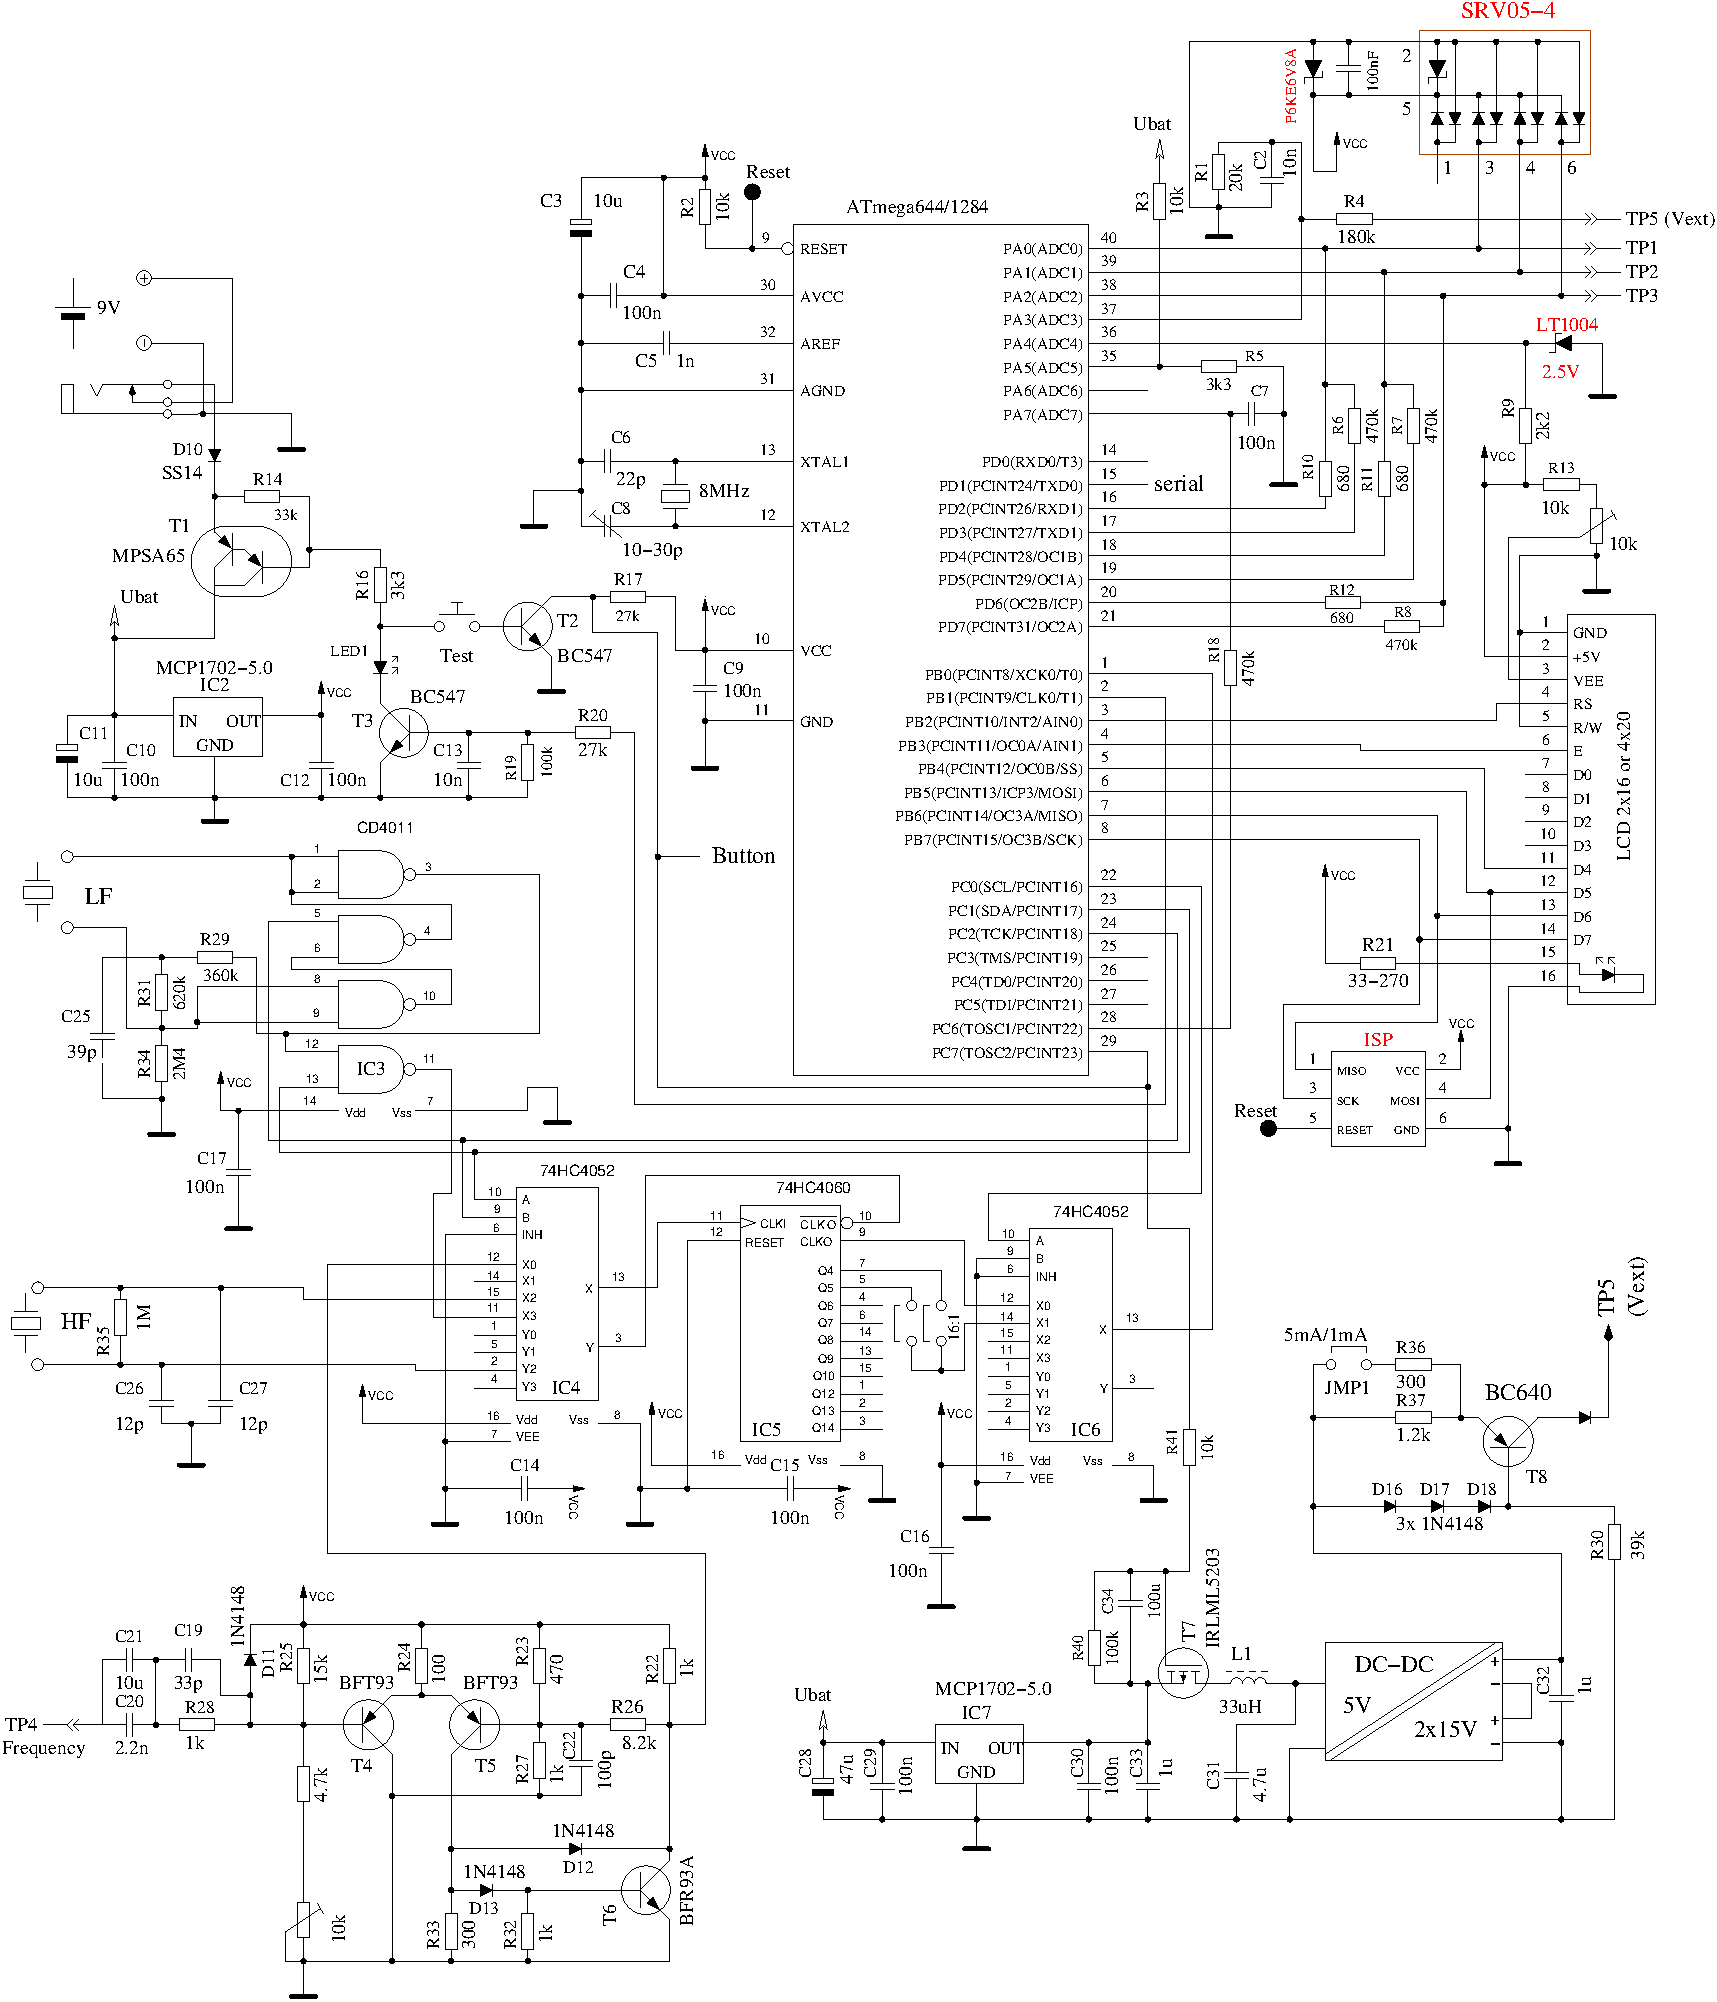
\includegraphics[width=1.\textwidth]{../FIG/t644tester.pdf}
\caption{Расширенная схема Транзистор Тестера с ATmega644}
\label{fig:t644tester}
\end{figure}

\begin{table}[H]
  \begin{center}
    \begin{tabular}{| c || c | c | c | c |}
    \hline
      Порт & Символьный & Графический LCD & Графический LCD & Дополнительные\\
	   &     LCD    &   SPI 4-wire &   I\textsuperscript{2}C      &  функции \\
    \hline
    \hline
    PB2    &  LCD-RS         &            &          &       \\
    \hline                                              
    PB3    &  LCD-E          &  (LCD-CE)  &  LCD-SCL &       \\
    \hline                                              
    PB4    &  LCD-D4         &  LCD-REST  &  LCD-SDA &       \\
    \hline                                              
    PB5    &  LCD-D5         &  LCD-RS    &          & ISP-MOSI \\
           &                 &            &          & поворотный энкодер 2 \\
    \hline                                              
    PB6    &  LCD-D6         &  LCD-SCLK  &          & ISP-MISO \\
    \hline                                            
    PB7    &  LCD-D7         &  LCD-SI    &          & ISP-SCK  \\
           &                 &            &          & поворотный энкодер 1 \\
    \hline
    \end{tabular}
  \end{center}
  \caption{Подключения дисплеев к портам ATmega324/644/1284}
  \label{tab:mega644-display}
\end{table}

Вы также можете подключить дисплей с контроллером NT7108 (KS0108, S6B0108) к тестеру, собранному на ATmega644 или ATmega1284
используя небольшую схему подключения показанную на рисунке~\ref{fig:NT7108lcd_644}.
Вы также должны учитывать различие в назначении контактов дисплейных модулей с контроллерами NT7108, 
как показано в таблице~\ref{tab:NT7108types} на странице~\pageref{tab:NT7108types}.

\begin{figure}[H]
  \begin{subfigure}[b]{.5\textwidth}
    \centering
    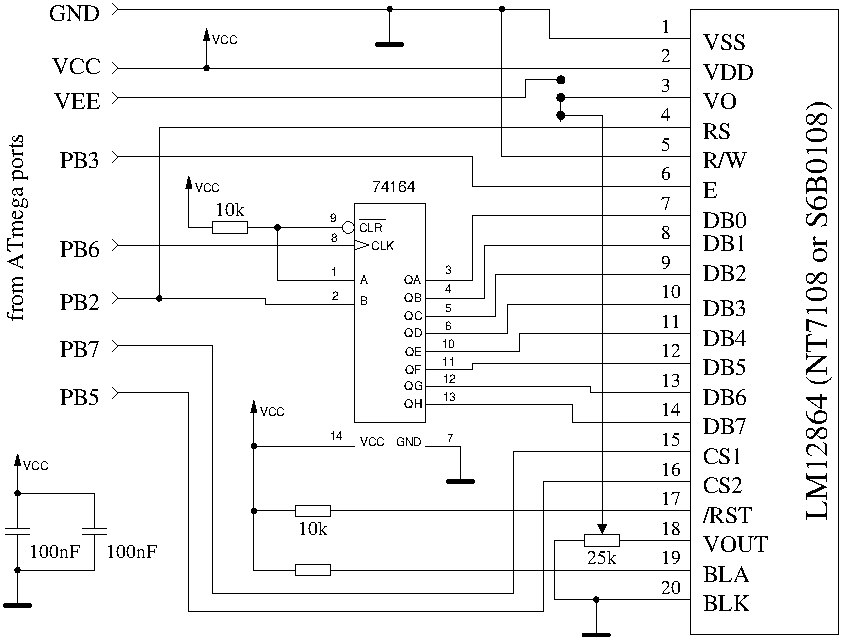
\includegraphics[width=.88\textwidth]{../FIG/ST7108serial164_644.pdf}
    \caption{при использовании 74HCT164}
  \end{subfigure}
  ~
  \begin{subfigure}[b]{.5\textwidth}
    \centering
    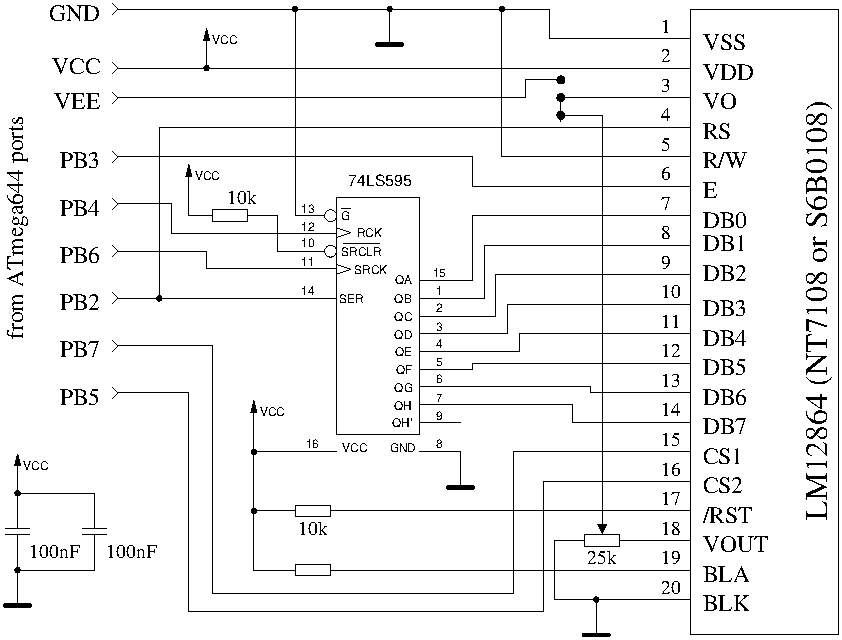
\includegraphics[width=.88\textwidth]{../FIG/ST7108serial595_644.pdf}
    \caption{при использовании 74HCT595}
  \end{subfigure}
  \caption{Подключение дисплея с контроллером NT7108 к ATmega644/1284}
  \label{fig:NT7108lcd_644}
\end{figure}

\section{Схема с использованием ATmega1280 или Arduino Mega}

Тестер может быть создан с использованием микроконтроллера ATmega1280 
или ATmega2560, а также построен на базе Arduino Mega.
Схема показана на рисунке~\ref{fig:t1280tester}.
Назначения контактов Arduino для подключения дисплея указаны зеленым цветом.
Компоненты, показанные красным цветом, не обязательны для правильной работы Тестера.
Контроллер ATmega2560 имеет большое количество портов, но только один порт
имеет функции, необходимые для обеих методик измерения частоты.
Порт должен быть одновременно таймером/счетчиком для подсчета внешних импульсов и
поддерживать внешнее прерывание при изменении уровня сигнала.
Этими функциями обладает только один порт PE6 (T3/INT6).
На остальных портах таймеров/счетчиков PD7 (T0), PD6 (T1), PH7 (T4) и PL2 (T5) отсутствует
внешнее прерывание.
К сожалению, порт PE6 не подключен к ленточному гнезду Arduino. 
Порт PE5 (вывод~7) подключен к контакту 3 разъема ШИМ и перемычкой 
может быть соединен с портом PE6 (вывод~8) ATmega2560.
Выходной сигнал генератора частоты можно получить на порту PB6 (OC1B).
Это порт подключен к контакту 12 разъема ШИМ.
ISP-разъем не требуется, так как программа может быть установлена при помощи  
загрузчика USB Arduino Mega. С использованием загрузчика есть небольшая задержка 
запуска программы.

\begin{figure}[H]
\centering
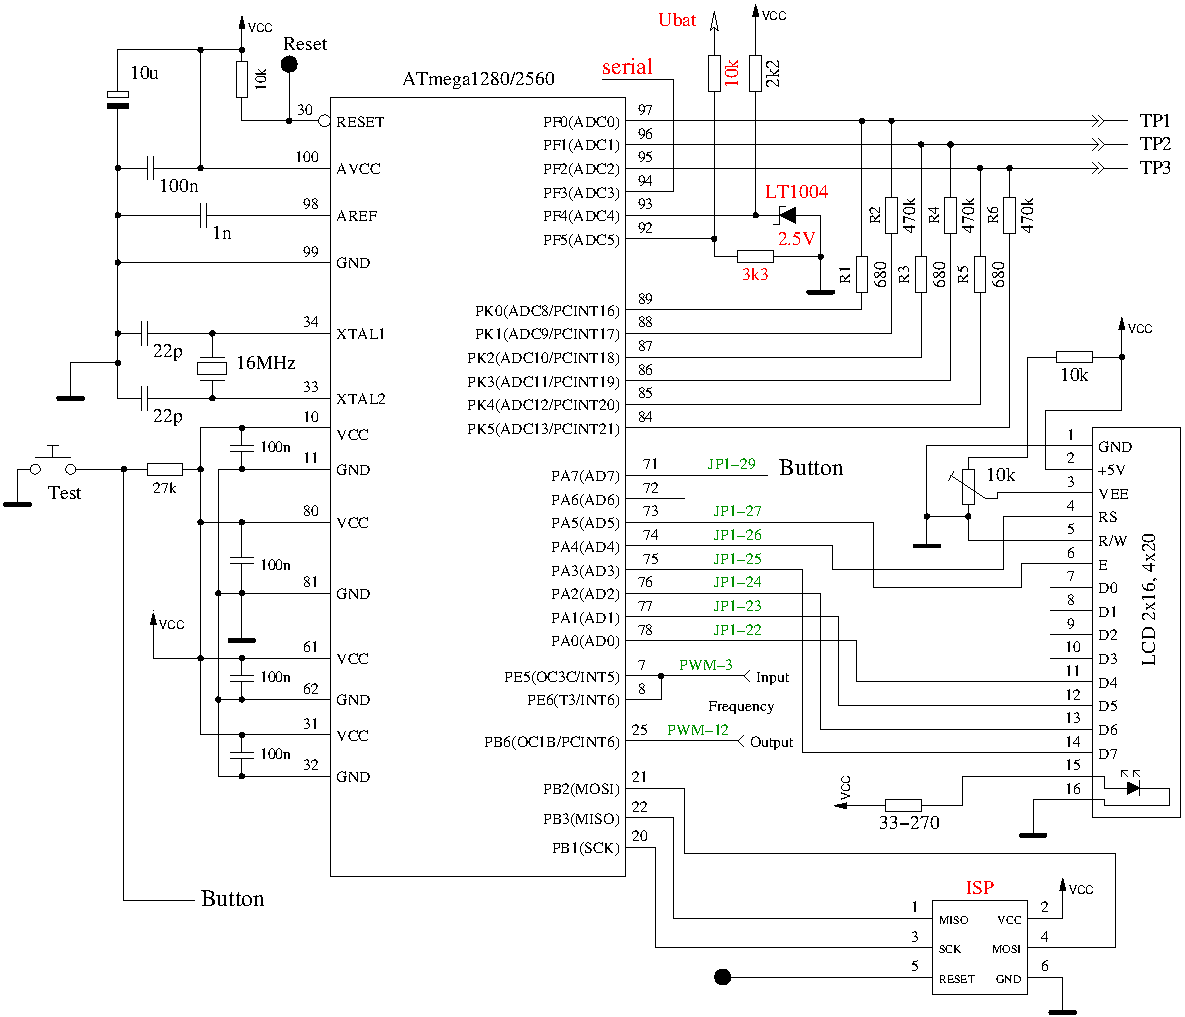
\includegraphics[width=1.\textwidth]{../FIG/t1280tester.pdf}
\caption{Схема Тестера с использованием ATmega1280, ATmega2560 или Arduino Mega}
\label{fig:t1280tester}
\end{figure}

Конечно, Вы можете подключить все поддерживаемые дисплеи и к ATmega1280 или ATmega2560
в соответствии с таблицей~\ref{tab:display-1280}.

\begin{table}[H]
  \begin{center}
    \begin{tabular}{| c || c | c | c | c | c | c |}
    \hline
      Порт & Символь-  &  ST7565     & ST7920       & NT7108       & SSD1306     & Дополнительные \\
           & ный LCD   &    SPI      & serial       & serial       & I\textsuperscript{2}C & функции \\
    \hline
    \hline
    PA0    &  LCD-D4   &   LCD-REST  &  LCD-RESET   & HC595-RCK      &             & \\
    \hline
    PA1    &  LCD-D5   &   LCD-RS    &              & LCD-CS2        &             & 2 канал энкодера \\
    \hline
    PA2    &  LCD-D6   &   LCD-SCLK  &              & HC164-CLK      &             & \\
    \hline
    PA3    &  LCD-D7   &   LCD-SI    &              & LCD-CS1        &             & 1 канал энкодера \\
    \hline
    PA4    &  LCD-RS   &             &   LCD-B0     & LCD-RS         &   LCD-SDA   & \\
           &           &             &              & HC164-SER      &             & \\
    \hline
    PA5    &  LCD-E    &   (LCD-CE)  &   LCD-EN     & LCD-EN         &   LCD--SCL  & \\
    \hline
    PA7    &  кнопка   &             &              &                &             & \\
    \hline
    \end{tabular}
  \end{center}
  \caption{Подключение различных дисплеев к ATmega1280/2560}
  \label{tab:display-1280}
\end{table}
\section{Китайские клоны с символьным дисплеем}
По имеющейся у меня информации, Тестер с символьным индикатором выпускают в Китае в двух версиях.
Первая модель первого дизайна от Markus F. 
без порта ISP. ATmega8 помещен в панельку, поэтому, Вы можете заменить его на ATmega168 или ATmega328. Для этой версии 
Вы должны рассмотреть все пункты раздела~\ref{sec:change_markus}.
Для лучшей стабилизации напряжения питания дополнительный керамический конденсатор на \(100~nF\) должен быть установлен 
поблизости VCC-GND и выводов AVCC-GND ATmega. Потому, что в тестере отсутствует разъем ISP, Вы должны его смонтировать
или использовать для программирования ATmega программатор с внешним разъемом.   
Кроме того, Вы должны иметь в виду, что, если Вы устанавливаете кварц 
на \(8~MHz\), то у Вашего внешнего программатора ISP должна быть частота синхронизации или кварц для программирования.\\

Вторая версия Тестера с элементами SMD. Там установлен ATmega168 в SMD корпусе 32TQFP. К счастью, установлен разъём ISP 
с 10 контактами для программирования. Я проанализировал версию платы \inquotes{2.1 2012/11/06}. Нашел одну ошибку - элемент \inquotes{D1}: 
установлен стабилитрон, а должен быть точный ИОН на \(2,5~V\). Стабилитрон необходимо удалить, а на его место установить 
ИОН LM4040AIZ2.5 или LT1004CZ-2.5. Недостающее опорное напряжение учитывается программным обеспечением даже, если ИОН 
не установлен. Мой образец был поставлен с программным обеспечением версии 1.02k. Разъём ISP с 10 контактами не был 
установлен, и я изготовил переходник от ISP6 к ISP10. У моего программатора цепь GND подведена к контакту 10, а на 
плате цепь GND подведена к контактам 4 и 6 ISP. Маркировка ATmega168 была стёрта, и не было никакой документации. 
Фьюзы блокировки ATmega были установлены таким образом, что бы считывание памяти было невозможно. Но установить 
программное обеспечение версии 1.05k удалось без проблем. У другого пользователя есть проблемы с программным 
обеспечением той же самой версии 1.05k. У этого пользователя китайская плата \inquotes{2.2 2012/11/26}. Программное обеспечение 
начинает работать, если установить дополнительный керамический конденсатор  \(100~nF\) между выводами AVCC (вывод 18) и 
GND (вывод 21) ATmega. Программное обеспечение версии 1.05k использует режим сна ATmega в течение времени ожидания 
измерения. По этой причине ток потребления изменяется часто и регулятор напряжения нагружается больше. Далее я заметил, 
что напряжение VCC блокировано керамическим конденсатором \(100~nF\) и электролитическим конденсатором
\(220~\mu F\) поблизости от 78L05. Входное напряжение \(9~V\) блокировано теми же самыми конденсаторами, но не на входе 
стабилизатора, а в эмиттере P-N-P-транзистора (параллельно батарее). Дорожка от ATmega168 до испытательного порта 
настолько тонкая, что сопротивление \(100~m\Omega\) не сможет быть измерено. Это будет причиной измерения сопротивления 
минимум \(0,3~\Omega\) для двух соединённых выводов. При измерении ESR эту величину обычно можно скомпенсировать. 
Программное обеспечение, начиная с версии 1.07k, учитывает это смещение для того, чтобы измерять резисторы 
сопротивлением ниже \(10~\Omega\).
\section{Китайские клоны с графическим дисплеем}
Новые сборки тестера, как, например, версия от Fish8840 используют 128x64 точки графический дисплей.
Эта версия использует модифицированную логику управления питанием и кнопками. 
Рисунок~\ref{fig:Fish8840} показывает часть модифицированной схемы.
\begin{figure}[H]
\centering
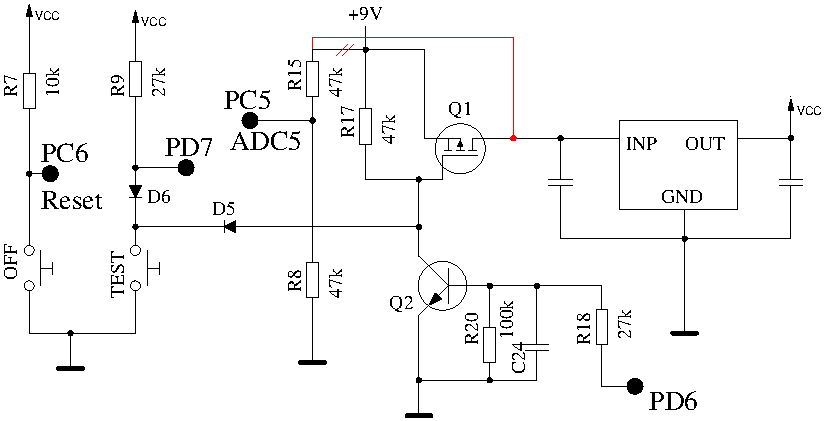
\includegraphics[width=.7\textwidth]{../FIG/Fish8840.pdf}
\caption{Часть схемы версии от Fish8840}
\label{fig:Fish8840}
\end{figure}
Как Вы можете видеть, вместо исходного коэффициента делителя, соотношение сопротивлений резисторов в цепи измерения 
напряжения батареи, R8 и R15 выбрано 2:1.
Кроме того, резистор R15 соединен непосредственно с батареей, что приводит к потреблению энергии в выключенном состоянии. 
Резистор R15 должен быть подключен к стоку Q1 или на вход регулятора напряжения для предотвращения ненужного 
расхода энергии батареи.
Соответствующие изменения в печатной плате изображены на рисунке~\ref{fig:Fish8840patch}.
Резистор R15 отсоединён от дорожки, идущей от R17 к D5 и при помощи эмалированной проволоки подсоединён к стоку Q1.
\begin{figure}[H]
\centering
\includegraphics[width=.7\textwidth]{../PNG/Fish8840patch.jpg}
\caption{Вариант изменения в печатной плате Fish8840}
\label{fig:Fish8840patch}
\end{figure}
Коэффициент делителя для измерения напряжения батареи должен быть задан в \lname{Makefile} (например: BAT\_NUMERATOR=66) 
после внесения изменений в оригинальное программное обеспечение.

Для адаптации рабочего напряжения к напряжению контроллера дисплея, модуль дисплея тестера Fish8840 
оснащен регулятором напряжения \(3,3~V\). 
Уровень логических сигналов от ATmega -- \(5~V\). Для адаптации уровня логических
сигналов ATmega к уровню сигналов контроллера дисплея рекомендуется адаптер, изображенный на рисунке~\ref{fig:Fish8840Adapt}.
Сигнальные линии четырех данных оснащены четырьмя резисторами \(2.7~k\Omega\) подсоединёнными последовательно 
для каждого сигнала на небольшой макетной плате. Для подсоединения платы дисплея к плате тестера Fish8840, в 
этом случае, необходимо использовать более длинные или дополнительные межплатные дистанцирующие стойки.
\begin{figure}[H]
  \begin{subfigure}[b]{.5\textwidth}
    \centering
    \includegraphics[width=1.\textwidth]{../PNG/Fish8840Adapt1.jpg}
    \caption{Вид дисплея с адаптером}
  \end{subfigure}
  ~
  \begin{subfigure}[b]{.5\textwidth}
    \centering
    \includegraphics[width=1.\textwidth]{../PNG/Fish8840Adapt2.jpg}
    \caption{Полностью собранный Тестер}
  \end{subfigure}
  \caption{Адаптер для коррекции подключения дисплея}
  \label{fig:Fish8840Adapt}
\end{figure}
Вместо приведенной выше модификации, Вы можете также использовать специальный режим вывода сигналов 
4~SPI ATmega, задав опцию в \lname{Makefile} LCD\_SPI\_OPEN\_COL.
С помощью этой опции, выходы не достигают уровня VCC, так как во время выхода высокого уровня 
подключаются \inquotes{подтягивающие резисторы} на весь период высокого уровня.
Если опция PULLUP\_DISABLE задана, то необходимо установить дополнительный внешний резистор для
сигнала \inquotes{RESET} (PD0).
Поскольку сигналы данных никогда не достигают уровня VCC, уровень \(3,3~V\) контроллера дисплея не 
будет превышен.
В моей версии тестера Fish8840, все сигналы дисплея подключены напрямую к разъему дисплея.
Таким образом, Вы можете подготовить печатную плату для подключения символьного дисплея, если на ней установлен 
ответный разъем и потенциометр для регулировки уровня контрастности.
Однако контакт 15 для подсветки подключается непосредственно к VCC Тестера.
Если Вы подключаете дисплей по такой схеме, Вы должны проверить, наличие ограничительного резистора
подсветки на плате модуля дисплея.
Конечно, Вы должны скомпилировать программное обеспечение для такого подключения дисплея.
Такая аппаратная доработка проверена для платы Fish8840.\\

Все попытки изменить программное обеспечение Вы делаете на свой страх и риск.
Никаких гарантий не может быть дано по поддержанию новых версий.
К сожалению, исходная китайская микропрограмма не может быть сохранена 
из-за установленных битов защиты ATmega328. Так что нет способа вернуть прибор в исходное состояние.\\

Дополнительная версия с графическим дисплеем WEI\_M8 печатной платы изображена на рисунке~\ref{fig:WeiM8}. 
Эта сборка использует аккумулятор LiIon AA размера в качестве источника питания, который может быть 
заряжен от микро USB разъема. 
Эксплуатировать Тестер можно также без аккумулятора, при питании только от USB.
\begin{figure}[H]
\centering
\includegraphics[width=.7\textwidth]{../PNG/WEI_M8.JPG}
\caption{Китайский клон WEI\_M8}
\label{fig:WeiM8}
\end{figure}
Отрадно, что сигнальные линии дисплея (на плате адаптера) оснащены резисторами, включёнными 
последовательно. Вы можете увидеть резисторы на рисунке~\ref{fig:WeiM8int} слева.
Таким образом, Вы не должны бояться, что \(5~V\) сигналы ATmega могут вызвать чрезмерное 
увеличение предельного логического уровня \(3,3~V\) контроллера дисплея.
\begin{figure}[H]
  \begin{subfigure}[b]{.5\textwidth}
    \centering
    \includegraphics[width=1.\textwidth]{../PNG/WEI_M8_D.JPG}
    \caption{Плата адаптера дисплея}
  \end{subfigure}
  ~
  \begin{subfigure}[b]{.5\textwidth}
    \centering
    \includegraphics[width=1.\textwidth]{../PNG/WEI_M8_L.JPG}
    \caption{Основная плата}
  \end{subfigure}
  \caption{Тестер WEI\_M8 в разобранном виде}
  \label{fig:WeiM8int}
\end{figure}
При обновлении до версии 1.12k обнаружены некоторые проблемы.
Если установить Extended Fuse 0x04 (0xFC), как рекомендуется, некоторые измерения вызывали сброс
процессора из-за короткого провала напряжения \inquotes{Brown Out}.
Я добавил дополнительный керамический конденсатор \(4.7~\mu F\) по входу 
регулятора напряжения и \(10~\mu F\) керамический конденсатор на выходе (VCC) регулятора.
И до, и после обновления я заметил, что в биполярных транзисторах, на этой плате, определяется 
дифференциальный ток коллектора (ICEO или ICEs) около \(1\mu A\).
После замены неизвестного LDO регулятора напряжения на MCP1702-5002 этот эффект исчез. 
Рисунок~\ref{fig:WeiM8mod} показывает измененную печатную плату с конденсаторами и регулятором MCP1702, 
установленными навесным монтажом.
Если Вы не желаете прислушиваться к совету, Вы должны установить Extended Fuse 0x07 (0xFF)
для поддержания бесперебойной работы. С этой настройкой кратковременные провалы не будут обнаружены.
\begin{figure}[H]
\centering
\includegraphics[width=.7\textwidth]{../PNG/WEI_M8_modified.JPG}
\caption{Тестер WEI\_M8 после модификации}
\label{fig:WeiM8mod}
\end{figure}
Дополнительная китайская версия с графическим дисплеем -- тестер \inquotes{LCD-T4} 
на печатной плате с жёлтой маской.
Я снял дисплей для замены программного обеспечения на новую версию.
На правом рисунке~\ref{fig:T4_front} Вы можете увидеть в правом верхнем углу отверстия для установки 
ISP разъёма с правильной разводкой для 6-ти контактного подключения программатора.
Для программирования ATmega я не устанавливал штыревой разъём. Я только вставил штыревой разъем  
в отверстия и придержал разъём шлейфа во время программирования.
При таком способе штыревой разъём может быть легко удален и дисплей установлен на место для 
возвращения первоначального вида прибора.
Китайское программное обеспечение может быть заменено на версию 1.12k без каких-либо заметных проблем.
Установка Extended Fuse 0x04 (0xFC) для проверки сброса из-за короткого провала напряжения \inquotes{Brown Out}
каких либо сюрпризов не принесла.
\begin{figure}[H]
  \begin{subfigure}[b]{.5\textwidth}
    \centering
    \includegraphics[width=1.\textwidth]{../PNG/T4_front.JPG}
    \caption{В собранном виде}
  \end{subfigure}
  ~
  \begin{subfigure}[b]{.5\textwidth}
    \centering
    \includegraphics[width=1.\textwidth]{../PNG/T4_front_noLCD.JPG}
    \caption{Со снятым дисплеем}
  \end{subfigure}
  \caption{Внешний вид T4 тестера}
  \label{fig:T4_front}
\end{figure}
Вы можете увидеть стойки \(5~mm\) и обновленные кабели с зажимами измерения на 
фотографии задней стороны на рисунке~\ref{fig:T4_back}.
Поскольку сигналы данных для графического контроллера дисплея не имеют преобразователя
логических уровней (\(5~V\) -\textgreater \ \(3.3~V\)), рекомендуется установить опцию LCD\_SPI\_OPEN\_COL.
В связи с тем, что плата не может быть легко модернизирована \inquotes{pull-up} резисторы могут быть
использованы путем отключения опции PULLUP\_DISABLE в \lname{Makefile}.
Эта плата является меньше практичной для последних расширений, а также замену дисплея 
трудно реализовать.
\begin{figure}[H]
  \begin{subfigure}[b]{.5\textwidth}
    \centering
    \includegraphics[width=1.\textwidth]{../PNG/T4_back.JPG}
    \caption{Сторона компонентов}
  \end{subfigure}
  ~
  \begin{subfigure}[b]{.5\textwidth}
    \centering
    \includegraphics[width=1.\textwidth]{../PNG/T4_back_clips.JPG}
    \caption{С кабелями измерения}
  \end{subfigure}
  \caption{Обратная сторона T4 тестера}
  \label{fig:T4_back}
\end{figure}
Еще одна версия китайского клона с графическим дисплеем имеет название \inquotes{GM328}.
В этой версии адаптер графического индикатора подключен через 16-пиновый разъем к основной плате.
Порт PD5 ATmega подключен через вывод 6 разъема на CE (Chip Enable) вход 
графического контроллера.
Сигнал СЕ также подключен к \(0~V\) (GND) на плате адаптера.
Результатом такого подключения будет короткое замыкание в случае переключения порта PD5 ATmega на
выход \(5~V\).
В новых версиях программного обеспечения выводится сигнал CE, даже если он не является необходимым.
Для правильной работы \inquotes{GM328} тестера с новыми версиями, Вы должны отсоединить сигнал CE (порт PD5 ATmega)
от вывода 6 в разъеме графического адаптера.
\section{Китайские наборы с графическими дисплеями}
Появились две новые версии набора с графическим дисплеем и поворотным энкодером.
Первый набор использует дисплей с контроллером ST7565 или совместимым (128х64 пикселей).
В дополнение к поворотному энкодеру, предусмотрен вход для измерения частоты.
Для тестовых площадок используется 14-контактный разъем Textool, три контакта под пайку
терминалов для подключения кабелей и тестовые площадки для теста деталей SMD.
На фотографии~\ref{fig:Kit_mono} показан смонтированный прибор.
Один из двух нагрузочных конденсаторов кварца \(22~pF\) заменен триммером.
Триммером можно подстроить частоту генерации кварца для повышения точности в режиме частотомера и генератора.
\begin{figure}[H]
  \begin{subfigure}[b]{.5\textwidth}
    \centering
    \includegraphics[width=1.\textwidth]{../PNG/Kit_ST7565a.jpg}
    \caption{смонтированный вид}
  \end{subfigure}
  \begin{subfigure}[b]{.5\textwidth}
    \centering
    \includegraphics[width=1.\textwidth]{../PNG/Kit_ST7565b.jpg}
    \caption{со снятым дисплеем}
  \end{subfigure}
  \caption{Собранный набор с дисплеем 128х64 пикселей}
  \label{fig:Kit_mono}
\end{figure}
Позже появился набор, который использует цветной дисплей с контроллером ST7735 (160x128 пикселей), 
дополнительно оснащен входом для измерения напряжения и выходом для генератора частот.
Но выход генератора не буферизирован, он просто подключен параллельно к контакту ТР2.
Вольтметр может измерять положительное постоянное  напряжение до \(50~V\).
Преобразователь напряжения DC-DC для измерения стабилитронов не предусмотрен.
На фотографиях~\ref{fig:Kit_color} показан этот собранный набор.
Кроме того, в этой версии один нагрузочный конденсатор кварца \(22~pF\) заменен триммером (зеленого цвета).
\begin{figure}[H]
  \begin{subfigure}[b]{.5\textwidth}
    \centering
    \includegraphics[width=1.\textwidth]{../PNG/Kit_Color_a.jpg}
    \caption{смонтированный вид}
  \end{subfigure}
  ~
  \begin{subfigure}[b]{.5\textwidth}
    \centering
    \includegraphics[width=1.\textwidth]{../PNG/Kit_Color_b.jpg}
    \caption{со снятым дисплеем}
  \end{subfigure}
  \caption{Собранный набор с цветным 160x128 пикселей дисплеем}
  \label{fig:Kit_color}
\end{figure}
Оба набора используют ATmega328P в DIP корпусе с установкой в панельку и
не оснащены разъемом ISP для обновления более новыми версиями программного обеспечения.
Первый комплект использует только выводные компоненты для монтажа печатной платы.
Я получил результат измерения резисторов \(680~\Omega\) и \(470~k\Omega\) с допуском 0.1\%\ в
этом китайском комплекте.
Также в набор добавлен конденсатор \(220~nF\) для калибровки.
Комплект с цветным дисплеем оснащён разъемом для подключения внешнего источника питания постоянного тока
вместо \(9~V\) батареи.
Некоторые SMD компоненты были смонтированы на основной плате, так что собрать тестер 
из этого набора не сложная задача.
Небольшой недостаток версии с цветным дисплеем –- скорость вывода на экран.
Особенно это заметно при  перемещении по пунктам меню.
В любом случае, цветной дисплей имеет большее разрешение, что позволяет отобразить больше информации сразу.

Оба набора используют стабилизатор напряжения \(3.3~V\) для питания контроллера
дисплея на плате индикатора.
Только контактный разъем должен быть припаян на печатной плате дисплея.
В цветной версии набора используется буфер CD4050, для адаптации логических уровней сигнала.
Я не обнаружил каких-либо элементов для адаптации уровней сигнала на плате с дисплеем ST7565.
Вероятно, выбранная версия контроллера допускает уровни сигнала \(5~V\) с ATmega328.
Я не обнаружил защитные диоды на входе сигналов со стороны питания \(3.3~V\) для данного типа контроллера.
\section{И еще один клон из Hiland M644}
Эта реплика основана на принципиальной электрической схеме Ника Л. из Украины,
\\см. Иллюстрацию~\ref{fig:t644tester} на странице~\pageref{fig:t644tester}.\\
\textbf{ Тестер работает с кнопкой, которая является одновременно кнопкой и кодером.}
Предлагает следующие дополнения:

\begin{itemize} \setlength{\itemsep}{-0.5\baselineskip}
 \item частота измерения
 \item генератор f
 \item 10-битный ШИМ
 \item импульсный энкодер
 \item измерение кварца
\item Определение напряжения и десятков диодов (почти до 50В).
\end{itemize}
\vspace{-0.5\baselineskip}
Плата оснащена 8 МГц кварцем. 16 МГц кварц будет лучше
Модифицировать триммер (более точную частоту) сложно.
\\ Контакты для интерфейса ISP находятся в 6-контактном ряду отверстий под
подключаемый модуль дисплея, который занят следующим образом:\\
\textbf{ слева направо}: 1~-сброс; 2~-SCK; 3~-MISO; 4~-MOSI; 5~-+5V; 6~-GND.\\
Чтобы иметь возможность обновить тестер, вам нужен относительно простой кабель
можете создать себя.
При поставке испытательное основание с нулевым усилием соединяется с платой через соединительные планки.

В тестере, показанном ниже, основание было припаяно непосредственно, и полоса сокета сохранена с этим
Припаяны к существующему ленточному кабелю с разъемом и закреплены термоусадочной трубкой.   
\begin{figure}[H]
 \begin{overpic}[width=.64\textwidth]{../FIG/Kabel_Hiland.pdf}
  \color{black}
  \put(14,99){\makebox(0,0)[cb]{Программист}}
  \put(12,-3){\makebox(0,0)[cb]{сообщение разъем}}  
  \put(49,99){\makebox(0,0)[cb]{вид сверху}}
  \put(40,-3){\makebox(0,0)[cb]{ленточный кабель}}  
  \put(90,99){\makebox(0,0)[cb]{Тестер}}
  \put(90,-3){\makebox(0,0)[cb]{Сосуд}}  
 \end{overpic}
 \caption{6 и 10-контактный кабель для программирования}
 \label{fig:Kabel}
\end{figure}

\begin{figure}[H]
  \begin{subfigure}[b]{.47\textwidth}
    \centering
    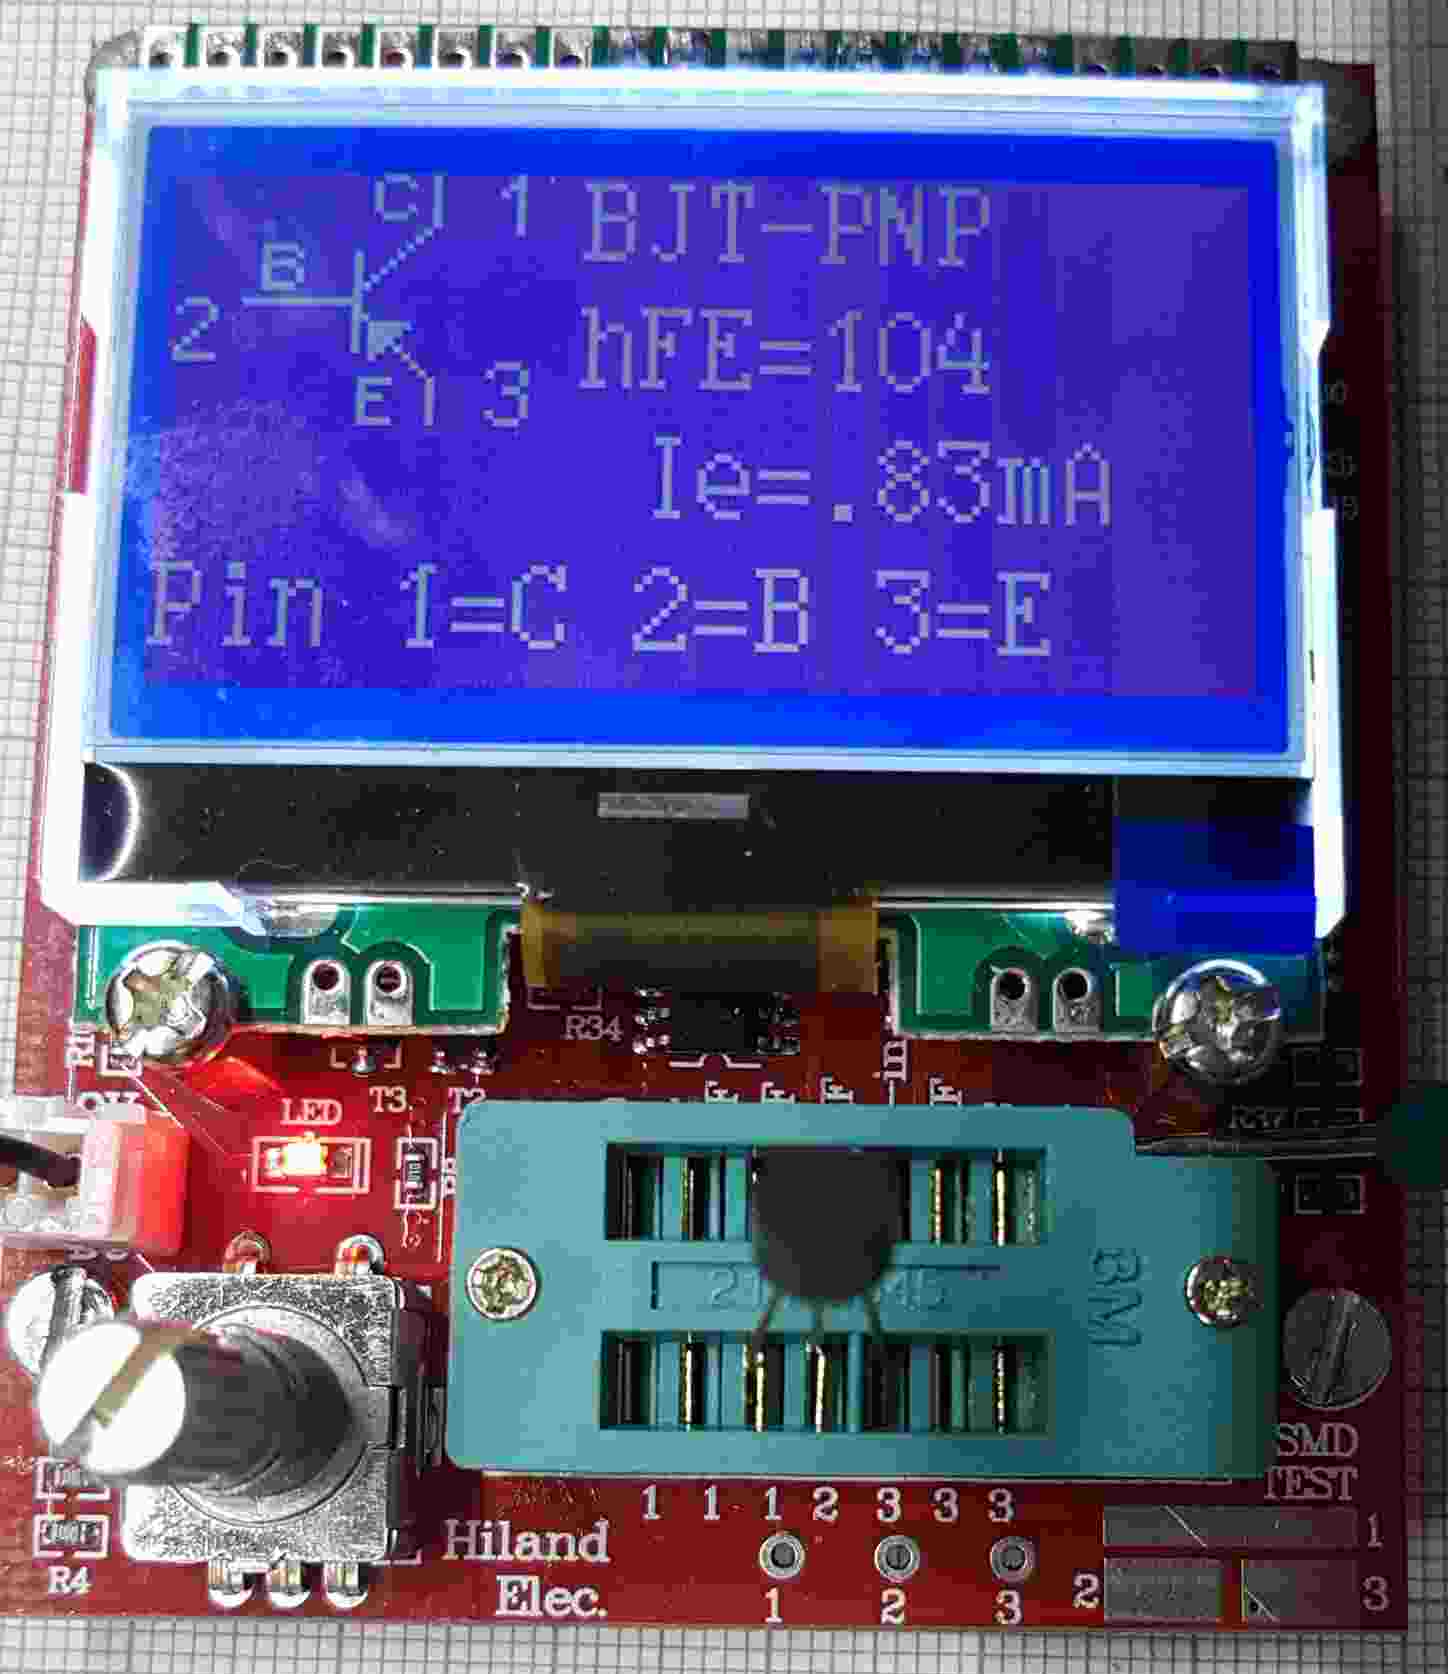
\includegraphics[width=.875\textwidth]{../PNG/Hi_u.jpg}
    \caption{ниже TP1 до TP3 для определения компонента}
  \end{subfigure}
  \begin{subfigure}[b]{.5\textwidth}
    \centering
    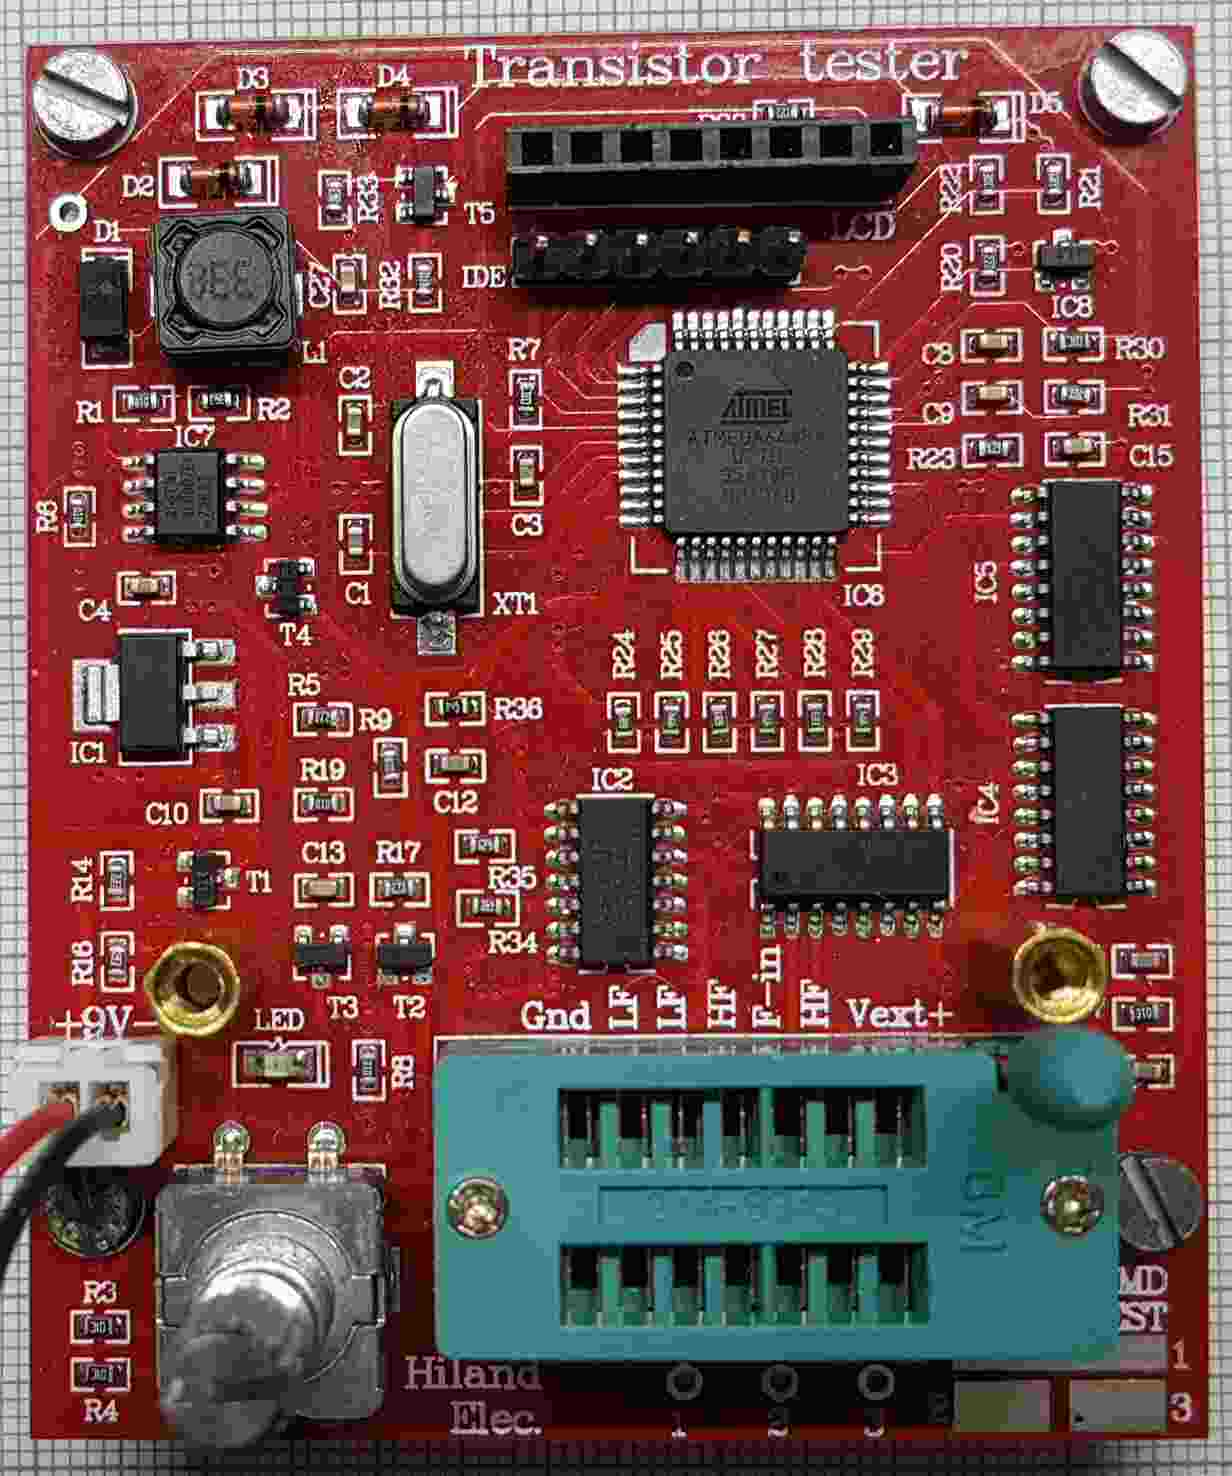
\includegraphics[width=.756\textwidth]{../PNG/Hi_o.jpg}
    \caption{штифты выше для меню выбора и IDE}
  \end{subfigure}
  \caption{Hiland Tester с тестовой базой и дисплеем 128 x 64 пикселей}
  \label{fig:Hiland}
\end{figure}

\textbf{ Тестовые порты TP1, TP2 и TP3}  используются для автоматического распознавания компонентов
и находятся на доске с номерами \textbf{1~~1~~1~~2~~3~~3~~3} в.

То же имя можно найти в поле теста SMD

и есть возможность паять свой собственный тестовый кабель.\\

\textbf{ Testport TP2} также используется для вывода специальной функции "f-Generator". \\
Контакты с маркировкой \textbf{ LF} предназначены для измерения кристаллов кварца с низкой резонансной частотой,
\\ и выводы с меткой \textbf{ HF} предназначены для кристаллов с высокой резонансной частотой.

Пин \textbf{ F-in} используется вместе с \textbf{ Gnd} для частоты специальной функции. \\
И вывод \textbf{ Vext+} также используется с \textbf{ Gnd} для измерения напряжения

\textbf{ и}  использует измерение стабилитрона.
